%
% This document contains the chapter some mathematical background.
%
% Copyright (C) 2003, 2004, 2005, 2006, 2007 Stefan Jahn <stefan@lkcc.org>
% Copyright (C) 2005, 2006
%               Michael Margraf <Michael.Margraf@alumni.TU-Berlin.DE>
%
% Permission is granted to copy, distribute and/or modify this document
% under the terms of the GNU Free Documentation License, Version 1.1
% or any later version published by the Free Software Foundation.
%

\chapter{Mathematical background}
%\addcontentsline{toc}{chapter}{Mathematical background}

\section{N-port matrix conversions}
%\addcontentsline{toc}{section}{Matrix conversions}
\label{sec:SparameterConversion}

When dealing with n-port parameters it may be necessary or
convenient to convert them into
other matrix representations used in electrical engineering.
The following matrices and notations are used in the
transformation equations.

\addvspace{12pt}

\begin{tabular}{rll}
$\left[\underline{X}\right]^{-1}$ & = & 
inverted matrix of $\left[\underline{X}\right]$\\& &\\
$\left[\underline{X}\right]^{*}$ & = & 
complex conjugated matrix of $\left[\underline{X}\right]$\\& &\\
$\left[\underline{E}\right]$ & = &
$\begin{bmatrix}
1 & 0 & \ldots & 0\\
0 & 1 & \ldots & 0\\
\vdots & \vdots & \ddots & \vdots\\
0 & 0 & \ldots & 1\\
\end{bmatrix}$
identity matrix\\& &\\
$\left[\underline{S}\right]$ & = & S-parameter matrix\\& &\\
$\left[\underline{Z}\right]$ & = & impedance matrix\\& &\\
$\left[\underline{Y}\right]$ & = & admittance matrix\\& &\\
$\left[\underline{Z}_{ref}\right]$ & = &
$\begin{pmatrix}
\underline{Z}_{0,1} & 0 & \ldots & 0\\
0 & \underline{Z}_{0,2} & \ldots & 0\\
\vdots & \vdots & \ddots & \vdots\\
0 & 0 & \ldots & \underline{Z}_{0,N}\\
\end{pmatrix}$\\& &\\
$\underline{Z}_{0,n}$ & = &
reference impedance of port $n$\\& &\\
$\left[G_{ref}\right]$ & = &
$\begin{pmatrix}
G_1 & 0 & \ldots & 0\\
0 & G_2 & \ldots & 0\\
\vdots & \vdots & \ddots & \vdots\\
0 & 0 & \ldots & G_N\\
\end{pmatrix}$\\& &\\
$G_n$ & = &
$\dfrac{1}{\sqrt{\text{Re}\left|\underline{Z}_{0,n}\right|}}$\\& &\\
\end{tabular}

\subsection{Renormalization of S-parameters to different port impedances}
%\addcontentsline{toc}{subsection}{Renormalization of S-parameters to different port impedances}

During S-parameter usage it sometimes appears to have not all components
in a circuit normalized to the same impedance. But calculations can only
be performed with all ports being normalized to the same impedance. In
the field of high frequency techniques this is usually $50\ohm$. In order
to transform to different port impedances, the following computation must
be applied to the resulting S-parameter matrix (valid only for real reference impedances).

\begin{equation}
\left[\underline{S'}\right] = \left[\underline{A}\right]^{-1} \cdot
\left(\left[\underline{S}\right] - \left[\underline{R}\right]\right) \cdot
\left(\left[\underline{E}\right] - \left[\underline{R}\right] \cdot \left[\underline{S}\right]\right)^{-1}
\cdot \left[\underline{A}\right]
\end{equation}

With

\addvspace{12pt}

\begin{tabular}{rll}
$Z_{n}$ & = & reference impedance of port $n$ after the normalizing process\\& &\\
$Z_{n,before}$ & = & reference impedance of port $n$ before the normalizing process\\& &\\
$\left[\underline{S}\right]$ & = & original S-parameter matrix\\& &\\
$\left[\underline{S'}\right]$ & = & recalculated scattering matrix\\& &\\
\end{tabular}

\begin{tabular}{rll}
$\left[\underline{R}\right]$ & = &
$\begin{pmatrix}
\underline{r}\left(Z_{1}\right) & 0 & \ldots & 0\\
0 & \underline{r}\left(Z_{2}\right) & \ldots & 0\\
\vdots & \vdots & \ddots & \vdots\\
0 & 0 & \ldots & \underline{r}\left(Z_{N}\right)\\
\end{pmatrix}$
reflection coefficient matrix\\& &\\
$\underline{r}\left(Z_{n}\right)$ & = &
$\dfrac{Z_{n} - Z_{n,before}}{Z_{n} + Z_{n,before}}$\\& &\\
$\left[\underline{A}\right]$ & = &
$\begin{pmatrix}
A_1 & 0 & \ldots & 0\\
0 & A_2 & \ldots & 0\\
\vdots & \vdots & \ddots & \vdots\\
0 & 0 & \ldots & A_N\\
\end{pmatrix}$\\& &\\
$A_n$ & = &
$\sqrt{\dfrac{Z_n}{Z_{n,before}}}\cdot\dfrac{2 Z_{n,before}}{Z_{n} + Z_{n,before}}$\\& &\\
\end{tabular}

\subsection{Transformations of n-Port matrices}
%\addcontentsline{toc}{subsection}{Transformations of n-Port matrices}

S-parameter, admittance and impedance matrices are not limited to One-
or Two-Port definitions.  They are defined for an arbitrary number of
ports.  The following section contains transformation formulas forth
and back each matrix representation.

\addvspace{12pt}

Converting a scattering parameter matrix to an impedance matrix is
done by the following formula.
\begin{align}
\left[
\underline{Z}
\right]
&=
\left[
\underline{G}_{ref}
\right]^{-1}
\cdot
\left(
\left[\underline{E}\right] - \left[\underline{S}\right]
\right)^{-1}
\cdot
\left(
\left[\underline{S}\right] \cdot \left[\underline{Z}_{ref}\right] + \left[\underline{Z}_{ref}\right]
\right)
\cdot
\left[\underline{G}_{ref}\right]\\
&=
\left[
\underline{G}_{ref}
\right]^{-1}
\cdot
\left(
\left[\underline{E}\right] - \left[\underline{S}\right]
\right)^{-1}
\cdot
\left(
\left[\underline{S}\right] + \left[\underline{E}\right]
\right)
\cdot \left[\underline{Z}_{ref}\right]
\cdot \left[\underline{G}_{ref}\right]
\end{align}

Converting a scattering parameter matrix to an admittance matrix can
be achieved by computing the following formula.
\begin{align}
\left[
\underline{Y}
\right]
&=
\left[
\underline{G}_{ref}
\right]^{-1}
\cdot
\left(
\left[\underline{S}\right] \cdot \left[\underline{Z}_{ref}\right] + \left[\underline{Z}_{ref}\right]
\right)^{-1}
\cdot
\left(
\left[\underline{E}\right] - \left[\underline{S}\right]
\right)
\cdot
\left[\underline{G}_{ref}\right]\\
&=
\left[\underline{G}_{ref}\right]^{-1}
\cdot \left[\underline{Z}_{ref}\right]^{-1}
\cdot
\left(
\left[\underline{S}\right] + \left[\underline{E}\right]
\right)^{-1}
\cdot
\left(
\left[\underline{E}\right] - \left[\underline{S}\right]
\right)
\cdot
\left[\underline{G}_{ref}\right]
\end{align}

Converting an impedance matrix to a scattering parameter matrix is
done by th following formula.
\begin{equation}
\left[
\underline{S}
\right]
=
\left[
\underline{G}_{ref}
\right]
\cdot
\left(
\left[\underline{Z}\right] - \left[\underline{Z}_{ref}\right]
\right)
\cdot
\left(
\left[\underline{Z}\right] + \left[\underline{Z}_{ref}\right]
\right)^{-1}
\cdot
\left[\underline{G}_{ref}\right]^{-1}
\end{equation}

Converting an admittance matrix to a scattering parameter matrix is
done by the following formula.
\begin{equation}
\label{eqn:Y2S}
\left[
\underline{S}
\right]
=
\left[
\underline{G}_{ref}
\right]
\cdot
\left(
\left[\underline{E}\right] - \left[\underline{Z}_{ref}\right] \cdot \left[\underline{Y}\right]
\right)
\cdot
\left(
\left[\underline{E}\right] + \left[\underline{Z}_{ref}\right] \cdot \left[\underline{Y}\right]
\right)^{-1}
\cdot
\left[\underline{G}_{ref}\right]^{-1}
\end{equation}

Converting an impedance matrix to an admittance matrix is done by the
following simple formula.
\begin{equation}
\left[
\underline{Y}
\right]
=
\left[
\underline{Z}
\right]^{-1}
\end{equation}

Converting an admittance matrix to an impedance matrix is done by the
following simple formula.
\begin{equation}
\left[
\underline{Z}
\right]
=
\left[
\underline{Y}
\right]^{-1}
\end{equation}

\subsection{Two-Port transformations}
%\addcontentsline{toc}{subsection}{Two-Port transformations}

\subsubsection{Two-Port matrix conversion based on current and voltage}
%\addcontentsline{toc}{subsubsection}{Two-Port matrix conversion based on current and voltage}

\begin{figure}[ht]
\begin{center}
\includegraphics[height=3cm]{twoportiv}
\end{center}
\caption{twoport definition using current and voltage}
\label{fig:twoportiv}
\end{figure}
\FloatBarrier

There are five different matrix forms for the correlations between the
quantities at the transmission twoport shown in
fig. \ref{fig:twoportiv}, each having its special meaning when
connecting twoports with each other.

\begin{itemize}

\item Y-parameters (also called admittance parameters)
\begin{equation}
\label{eq:yparamdef}
\begin{pmatrix}
\underline{I}_{1}\\
\underline{I}_{2}
\end{pmatrix}
=
\begin{pmatrix}
\underline{Y}_{11} & \underline{Y}_{12}\\
\underline{Y}_{21} & \underline{Y}_{22}
\end{pmatrix}
\cdot
\begin{pmatrix}
\underline{V}_{1}\\
\underline{V}_{2}
\end{pmatrix}
\end{equation}

\item Z-parameters (also called impedance parameters)
\begin{equation}
\label{eq:zparamdef}
\begin{pmatrix}
\underline{V}_{1}\\
\underline{V}_{2}
\end{pmatrix}
=
\begin{pmatrix}
\underline{Z}_{11} & \underline{Z}_{12}\\
\underline{Z}_{21} & \underline{Z}_{22}
\end{pmatrix}
\cdot
\begin{pmatrix}
\underline{I}_{1}\\
\underline{I}_{2}
\end{pmatrix}
\end{equation}

\item H-parameters (also called hybrid parameters)
\begin{equation}
\label{eq:hparamdef}
\begin{pmatrix}
\underline{V}_{1}\\
\underline{I}_{2}
\end{pmatrix}
=
\begin{pmatrix}
\underline{H}_{11} & \underline{H}_{12}\\
\underline{H}_{21} & \underline{H}_{22}
\end{pmatrix}
\cdot
\begin{pmatrix}
\underline{I}_{1}\\
\underline{V}_{2}
\end{pmatrix}
\end{equation}

\item G-parameters (also called C-parameters)
\begin{equation}
\label{eq:gparamdef}
\begin{pmatrix}
\underline{I}_{1}\\
\underline{V}_{2}
\end{pmatrix}
=
\begin{pmatrix}
\underline{G}_{11} & \underline{G}_{12}\\
\underline{G}_{21} & \underline{G}_{22}
\end{pmatrix}
\cdot
\begin{pmatrix}
\underline{V}_{1}\\
\underline{I}_{2}
\end{pmatrix}
\end{equation}

\item A-parameters (also called chain or ABCD-parameters)
\begin{equation}
\label{eq:aparamdef}
\begin{pmatrix}
\underline{V}_{1}\\
\underline{I}_{1}
\end{pmatrix}
=
\begin{pmatrix}
\underline{A}_{11} & \underline{A}_{12}\\
\underline{A}_{21} & \underline{A}_{22}
\end{pmatrix}
\cdot
\begin{pmatrix}
\underline{V}_{2}\\
-\underline{I}_{2}
\end{pmatrix}
\end{equation}

\end{itemize}

\begin{center}
\begin{figure}[ht]
\setlength{\fboxsep}{5pt}
\begin{tabular}{|c|c|c|c|}
\hline
\setlength{\fboxrule}{0pt}
\fbox{\begin{minipage}[t]{0.22\linewidth}
\centering
parallel-parallel connection\\[1ex]
\includegraphics[height=2.5cm]{twoportpp}
\end{minipage}}
&
\begin{minipage}[t]{0.21\linewidth}
\centering
series-series connection\\[1ex]
\includegraphics[height=2.5cm]{twoportss}
\end{minipage}
&
\begin{minipage}[t]{0.21\linewidth}
\centering
series-parallel connection\\[1ex]
\includegraphics[height=2.5cm]{twoportps}
\end{minipage}
&
\begin{minipage}[t]{0.21\linewidth}
\centering
parallel-series connection\\[1ex]
\includegraphics[height=2.5cm]{twoportsp}
\end{minipage}
\\
\hline
\multicolumn{4}{|c|}{
\setlength{\fboxrule}{0pt}
\fbox{\begin{minipage}[t]{0.85\linewidth}
\centering
cascaded twoports\\[1ex]
\includegraphics[height=1.3cm]{twoportch}
\end{minipage}}
}
\\
\hline
\end{tabular}
\end{figure}
\FloatBarrier
\end{center}

Basically there are five different kinds of twoport connections.
Using the corresponding twoport matrix representations, complicated
networks can be analysed by connecting elementary twoports.  The
linear correlations between the complex currents and voltages rms
values of a twoport are described by four complex twoport parameters
(i.e. the twoport matrix).  These parameters are used to describe the
AC behaviour of the twoport.

\begin{itemize}
\item parallel-parallel connection: use Y-parameters: $Y = Y_{1} + Y_{2}$
\item series-series connection: use Z-parameters: $Z = Z_{1} + Z_{2}$
\item series-parallel connection: use H-parameters: $H = H_{1} + H_{2}$
\item parallel-series connection: use G-parameters: $G = G_{1} + G_{2}$
\item chain connection: use A-parameters: $A = A_{1}\cdot A_{2}$
\end{itemize}

\setlength{\fboxsep}{4pt}
\def\a{0.15\linewidth}
\begin{tabular}{|c|c|c|c|c|c|}
\hline
& A & Y & Z & H & G\\
\hline
A & 
\makebox[\a][c]{$\begin{array}{cc}A_{11}&A_{12}\vspace{4pt}\\A_{21}&A_{22}\end{array}$} &
\setlength{\fboxrule}{0pt}
\fbox{\makebox[\a][c]{$\begin{array}{cc}\dfrac{-Y_{22}}{Y_{21}}&\dfrac{-1}{Y_{21}}\vspace{4pt}\\\dfrac{-\Delta Y}{Y_{21}}&\dfrac{-Y_{11}}{Y_{21}}\end{array}$}} &
\makebox[\a][c]{$\begin{array}{cc}\dfrac{Z_{11}}{Z_{21}}&\dfrac{\Delta Z}{Z_{21}}\vspace{4pt}\\\dfrac{1}{Z_{21}}&\dfrac{Z_{22}}{Z_{21}}\end{array}$} &
\makebox[\a][c]{$\begin{array}{cc}\dfrac{-\Delta H}{H_{21}}&\dfrac{-H_{11}}{H_{21}}\vspace{4pt}\\\dfrac{-H_{22}}{H_{21}}&\dfrac{-1}{H_{21}}\end{array}$} &
\makebox[\a][c]{$\begin{array}{cc}\dfrac{1}{G_{21}}&\dfrac{G_{22}}{G_{21}}\vspace{4pt}\\\dfrac{G_{11}}{G_{21}}&\dfrac{\Delta G}{G_{21}}\end{array}$}\\
\hline
Y & 
\setlength{\fboxrule}{0pt}
\fbox{\makebox[\a][c]{$\begin{array}{cc}\dfrac{A_{22}}{A_{12}}&\dfrac{-\Delta A}{A_{12}}\vspace{4pt}\\\dfrac{-1}{A_{12}}&\dfrac{A_{11}}{A_{12}}\end{array}$}} &
\makebox[\a][c]{$\begin{array}{cc}Y_{11}&Y_{12}\vspace{4pt}\\Y_{21}&Y_{22}\end{array}$} & 
\makebox[\a][c]{$\begin{array}{cc}\dfrac{Z_{22}}{\Delta Z}&\dfrac{-Z_{12}}{\Delta Z}\vspace{4pt}\\\dfrac{-Z_{21}}{\Delta Z}&\dfrac{Z_{11}}{\Delta Z}\end{array}$} &
\makebox[\a][c]{$\begin{array}{cc}\dfrac{1}{H_{11}}&\dfrac{-H_{12}}{H_{11}}\vspace{4pt}\\\dfrac{H_{21}}{H_{11}}&\dfrac{\Delta H}{H_{11}}\end{array}$} &
\makebox[\a][c]{$\begin{array}{cc}\dfrac{\Delta G}{G_{22}}&\dfrac{G_{12}}{G_{22}}\vspace{4pt}\\\dfrac{-G_{21}}{G_{22}}&\dfrac{1}{G_{22}}\end{array}$}\\
\hline
Z & 
\setlength{\fboxrule}{0pt}
\fbox{\makebox[\a][c]{$\begin{array}{cc}\dfrac{A_{11}}{A_{21}}&\dfrac{\Delta A}{A_{21}}\vspace{4pt}\\\dfrac{1}{A_{21}}&\dfrac{A_{22}}{A_{21}}\end{array}$}} &
\makebox[\a][c]{$\begin{array}{cc}\dfrac{Y_{22}}{\Delta Y}&\dfrac{-Y_{12}}{\Delta Y}\vspace{4pt}\\\dfrac{-Y_{21}}{\Delta Y}&\dfrac{Y_{11}}{\Delta Y}\end{array}$} &
\makebox[\a][c]{$\begin{array}{cc}Z_{11}&Z_{12}\vspace{4pt}\\Z_{21}&Z_{22}\end{array}$} & 
\makebox[\a][c]{$\begin{array}{cc}\dfrac{\Delta H}{H_{22}}&\dfrac{H_{12}}{H_{22}}\vspace{4pt}\\\dfrac{-H_{21}}{H_{22}}&\dfrac{1}{H_{22}}\end{array}$} &
\makebox[\a][c]{$\begin{array}{cc}\dfrac{1}{G_{11}}&\dfrac{-G_{12}}{G_{11}}\vspace{4pt}\\\dfrac{G_{21}}{G_{11}}&\dfrac{\Delta G}{G_{11}}\end{array}$}\\
\hline
H & 
\setlength{\fboxrule}{0pt}
\fbox{\makebox[\a][c]{$\begin{array}{cc}\dfrac{A_{12}}{A_{22}}&\dfrac{\Delta A}{A_{22}}\vspace{4pt}\\\dfrac{-1}{A_{22}}&\dfrac{A_{21}}{A_{22}}\end{array}$}} &
\makebox[\a][c]{$\begin{array}{cc}\dfrac{1}{Y_{11}}&\dfrac{-Y_{12}}{Y_{11}}\vspace{4pt}\\\dfrac{Y_{21}}{Y_{11}}&\dfrac{\Delta Y}{Y_{11}}\end{array}$} &
\makebox[\a][c]{$\begin{array}{cc}\dfrac{\Delta Z}{Z_{22}}&\dfrac{Z_{12}}{Z_{22}}\vspace{4pt}\\\dfrac{-Z_{21}}{Z_{22}}&\dfrac{1}{Z_{22}}\end{array}$} &
\makebox[\a][c]{$\begin{array}{cc}H_{11}&H_{12}\vspace{4pt}\\H_{21}&H_{22}\end{array}$} & 
\makebox[\a][c]{$\begin{array}{cc}\dfrac{G_{22}}{\Delta G}&\dfrac{-G_{12}}{\Delta G}\vspace{4pt}\\\dfrac{-G_{21}}{\Delta G}&\dfrac{G_{11}}{\Delta G}\end{array}$}\\
\hline
G & 
\setlength{\fboxrule}{0pt}
\fbox{\makebox[\a][c]{$\begin{array}{cc}\dfrac{A_{21}}{A_{11}}&\dfrac{-\Delta A}{A_{11}}\vspace{4pt}\\\dfrac{1}{A_{11}}&\dfrac{A_{12}}{A_{11}}\end{array}$}} &
\makebox[\a][c]{$\begin{array}{cc}\dfrac{\Delta Y}{Y_{22}}&\dfrac{Y_{12}}{Y_{22}}\vspace{4pt}\\\dfrac{-Y_{21}}{Y_{22}}&\dfrac{1}{Y_{22}}\end{array}$} &
\makebox[\a][c]{$\begin{array}{cc}\dfrac{1}{Z_{11}}&\dfrac{-Z_{12}}{Z_{11}}\vspace{4pt}\\\dfrac{Z_{21}}{Z_{11}}&\dfrac{\Delta Z}{Z_{11}}\end{array}$} &
\makebox[\a][c]{$\begin{array}{cc}\dfrac{H_{22}}{\Delta H}&\dfrac{-H_{12}}{\Delta H}\vspace{4pt}\\\dfrac{-H_{21}}{\Delta H}&\dfrac{H_{11}}{\Delta H}\end{array}$} &
\makebox[\a][c]{$\begin{array}{cc}G_{11}&G_{12}\vspace{4pt}\\G_{21}&G_{22}\end{array}$}\\
\hline
\end{tabular}

\subsubsection{Two-Port matrix conversion based on signal waves}
%\addcontentsline{toc}{subsubsection}{Two-Port matrix conversion based on signal waves}

\begin{figure}[ht]
\begin{center}
\includegraphics[height=3cm]{twoportab}
\end{center}
\caption{twoport definition using signal waves}
\label{fig:twoportab}
\end{figure}
\FloatBarrier

There are two different matrix forms for the correlations between the
quantities at the transmission twoport shown in
fig. \ref{fig:twoportab}.

\begin{itemize}

\item S-parameters (also called scattering parameters)
\begin{equation}
\label{eq:sparamdef}
\begin{pmatrix}
\underline{b}_{1}\\
\underline{b}_{2}
\end{pmatrix}
=
\begin{pmatrix}
\underline{S}_{11} & \underline{S}_{12}\\
\underline{S}_{21} & \underline{S}_{22}
\end{pmatrix}
\cdot
\begin{pmatrix}
\underline{a}_{1}\\
\underline{a}_{2}
\end{pmatrix}
\end{equation}

\item T-parameters (also called transfer scattering parameters)
\begin{equation}
\label{eq:tparamdef}
\begin{pmatrix}
\underline{a}_{1}\\
\underline{b}_{1}
\end{pmatrix}
=
\begin{pmatrix}
\underline{T}_{11} & \underline{T}_{12}\\
\underline{T}_{21} & \underline{T}_{22}
\end{pmatrix}
\cdot
\begin{pmatrix}
\underline{b}_{2}\\
\underline{a}_{2}
\end{pmatrix}
\end{equation}

\end{itemize}

When connecting cascaded twoports it is possible to compute the
resulting transfer scattering parameters by the following equation.
\begin{equation}
T = T_1 \cdot T_2
\end{equation}

According to Janusz A. Dobrowolski \cite{Dobrowolski} the following
table contains the matrix transformation formulas.

\addvspace{12pt}

\begin{tabular}{|c|c|c|}
\hline
& S & T\\
\hline
S &
$\begin{array}{cc}S_{11}&S_{12}\vspace{4pt}\\S_{21}&S_{22}\end{array}$ &
\setlength{\fboxrule}{0pt}
\fbox{$\begin{array}{cc}\dfrac{T_{12}}{T_{22}}&\dfrac{\Delta T}{T_{22}}\vspace{4pt}\\\dfrac{1}{T_{22}}&\dfrac{-T_{21}}{T_{22}}\end{array}$}\\
\hline
T &
\setlength{\fboxrule}{0pt}
\fbox{$\begin{array}{cc}\dfrac{-\Delta S}{S_{21}}&\dfrac{S_{11}}{S_{21}}\vspace{4pt}\\\dfrac{-S_{22}}{S_{21}}&\dfrac{1}{S_{21}}\end{array}$} &
$\begin{array}{cc}T_{11}&T_{12}\vspace{4pt}\\T_{21}&T_{22}\end{array}$\\
\hline
\end{tabular}

\subsubsection{Mixed Two-Port matrix conversions}
%\addcontentsline{toc}{subsubsection}{Mixed Two-Port matrix conversions}

Sometimes it may be useful to have a twoport matrix representation
based on signal waves in a representation based on voltage and current
and the other way around.  There are two more parameters involved in
this case: The reference impedance at port 1 (denoted as $Z_1$) and
the reference impedance at port 2 (denoted as $Z_2$).

\addvspace{12pt}

Converting from scattering parameters to chain parameters results in
\begin{align}
A_{11} &= \dfrac{Z_{1}^{*} + Z_{1}\cdot S_{11} - Z_{1}^{*}\cdot S_{22} - Z_{1}\cdot \Delta S}{2\cdot S_{21}\cdot \sqrt{Re\left(Z_{1}\right)\cdot Re\left(Z_{2}\right)}}\\
A_{12} &= \dfrac{Z_{1}^{*}\cdot Z_{2}^{*} + Z_{1}\cdot Z_{2}^{*}\cdot S_{11} + Z_{1}^{*}\cdot Z_{2}\cdot S_{22} + Z_{1}\cdot Z_{2}\cdot \Delta S}{2\cdot S_{21}\cdot \sqrt{Re\left(Z_{1}\right)\cdot Re\left(Z_{2}\right)}}\\
A_{21} &= \dfrac{1 - S_{11} - S_{22} + \Delta S}{2\cdot S_{21}\cdot \sqrt{Re\left(Z_{1}\right)\cdot Re\left(Z_{2}\right)}}\\
A_{22} &= \dfrac{Z_{2}^{*} - Z_{2}^{*}\cdot S_{11} + Z_{2}\cdot S_{22} - Z_{2}\cdot \Delta S}{2\cdot S_{21}\cdot \sqrt{Re\left(Z_{1}\right)\cdot Re\left(Z_{2}\right)}}\\
%\end{align}
\intertext{
Converting from chain parameters to scattering parameters results in
}
%\begin{align}
S_{11} &= \dfrac{A_{11}\cdot Z_{2} + A_{12} - A_{21}\cdot Z_{1}^{*}\cdot Z_{2} - A_{22}\cdot Z_{1}^{*}}{A_{11}\cdot Z_{2} + A_{12} + A_{21}\cdot Z_{1}\cdot Z_{2} + A_{22}\cdot Z_{1}}\\
S_{12} &= \dfrac{\Delta A\cdot 2\cdot \sqrt{Re\left(Z_{1}\right)\cdot Re\left(Z_{2}\right)}}{A_{11}\cdot Z_{2} + A_{12} + A_{21}\cdot Z_{1}\cdot Z_{2} + A_{22}\cdot Z_{1}}\\
S_{21} &= \dfrac{2\cdot \sqrt{Re\left(Z_{1}\right)\cdot Re\left(Z_{2}\right)}}{A_{11}\cdot Z_{2} + A_{12} + A_{21}\cdot Z_{1}\cdot Z_{2} + A_{22}\cdot Z_{1}}\\
S_{22} &= \dfrac{-A_{11}\cdot Z_{2}^{*} + A_{12} - A_{21}\cdot Z_{1}\cdot Z_{2}^{*} + A_{22}\cdot Z_{1}}{A_{11}\cdot Z_{2} + A_{12} + A_{21}\cdot Z_{1}\cdot Z_{2} + A_{22}\cdot Z_{1}}
\end{align}

Converting from scattering parameters to hybrid parameters results in
\begin{align}
H_{11} &= Z_{1}\cdot \dfrac{\left(1 + S_{11}\right)\cdot \left(1 + S_{22}\right) - S_{12}\cdot S_{21}}{\left(1 - S_{11}\right)\cdot \left(1 + S_{22}\right) + S_{12}\cdot S_{21}}\\
H_{12} &= \sqrt{\dfrac{Z_1}{Z_2}}\cdot \dfrac{2\cdot S_{12}}{\left(1 - S_{11}\right)\cdot \left(1 + S_{22}\right) + S_{12}\cdot S_{21}}\\
H_{21} &= \sqrt{\dfrac{Z_1}{Z_2}}\cdot \dfrac{-2\cdot S_{21}}{\left(1 - S_{11}\right)\cdot \left(1 + S_{22}\right) + S_{12}\cdot S_{21}}\\
H_{22} &= \dfrac{1}{Z_{2}}\cdot \dfrac{\left(1 - S_{11}\right)\cdot \left(1 - S_{22}\right) - S_{12}\cdot S_{21}}{\left(1 - S_{11}\right)\cdot \left(1 + S_{22}\right) + S_{12}\cdot S_{21}}\\
\intertext{
Converting from hybrid parameters to scattering parameters results in
}
S_{11} &= \dfrac{\left(H_{11} - Z_{1}\right)\cdot \left(1 + Z_{2}\cdot H_{22}\right) - Z_2\cdot H_{12}\cdot H_{21}}{\left(H_{11} + Z_{1}\right)\cdot \left(1 + Z_{2}\cdot H_{22}\right) - Z_2\cdot H_{12}\cdot H_{21}}\\
S_{12} &= \dfrac{2\cdot H_{12}\cdot\sqrt{Z_1\cdot Z_2}}{\left(H_{11} + Z_{1}\right)\cdot \left(1 + Z_{2}\cdot H_{22}\right) - Z_2\cdot H_{12}\cdot H_{21}}\\
S_{21} &= \dfrac{-2\cdot H_{21}\cdot\sqrt{Z_1\cdot Z_2}}{\left(H_{11} + Z_{1}\right)\cdot \left(1 + Z_{2}\cdot H_{22}\right) - Z_2\cdot H_{12}\cdot H_{21}}\\
S_{22} &= \dfrac{\left(H_{11} + Z_{1}\right)\cdot \left(1 - Z_{2}\cdot H_{22}\right) + Z_2\cdot H_{12}\cdot H_{21}}{\left(H_{11} + Z_{1}\right)\cdot \left(1 + Z_{2}\cdot H_{22}\right) - Z_2\cdot H_{12}\cdot H_{21}}
\end{align}

Converting from scattering parameters to the second type of hybrid
parameters results in
\begin{align}
G_{11} &= \dfrac{1}{Z_{1}}\cdot \dfrac{\left(1 - S_{11}\right)\cdot \left(1 - S_{22}\right) - S_{12}\cdot S_{21}}{\left(1 + S_{11}\right)\cdot \left(1 - S_{22}\right) + S_{12}\cdot S_{21}}\\
G_{12} &= \sqrt{\dfrac{Z_2}{Z_1}}\cdot \dfrac{-2\cdot S_{12}}{\left(1 + S_{11}\right)\cdot \left(1 - S_{22}\right) + S_{12}\cdot S_{21}}\\
G_{21} &= \sqrt{\dfrac{Z_2}{Z_1}}\cdot \dfrac{2\cdot S_{21}}{\left(1 + S_{11}\right)\cdot \left(1 - S_{22}\right) + S_{12}\cdot S_{21}}\\
G_{22} &= Z_{2}\cdot \dfrac{\left(1 + S_{11}\right)\cdot \left(1 + S_{22}\right) - S_{12}\cdot S_{21}}{\left(1 + S_{11}\right)\cdot \left(1 - S_{22}\right) + S_{12}\cdot S_{21}}\\
\intertext{
Converting from the second type of hybrid parameters to scattering
parameters results in
}
S_{11} &= \dfrac{\left(1 - G_{11}\cdot Z_{1}\right)\cdot \left(G_{22} + Z_{2}\right) + Z_1\cdot G_{12}\cdot G_{21}}{\left(1 + G_{11}\cdot Z_{1}\right)\cdot \left(G_{22} + Z_{2}\right) - Z_1\cdot G_{12}\cdot G_{21}}\\
S_{12} &= \dfrac{-2\cdot G_{12}\cdot\sqrt{Z_1\cdot Z_2}}{\left(1 + G_{11} \cdot Z_{1}\right)\cdot \left(G_{22} + Z_{2}\right) - Z_1\cdot G_{12}\cdot G_{21}}\\
S_{21} &= \dfrac{2\cdot G_{21}\cdot\sqrt{Z_1\cdot Z_2}}{\left(1 + G_{11} \cdot Z_{1}\right)\cdot \left(G_{22} + Z_{2}\right) - Z_1\cdot G_{12}\cdot G_{21}}\\
S_{22} &= \dfrac{\left(1 + G_{11} \cdot Z_{1}\right)\cdot \left(G_{22} - Z_{2}\right) - Z_1\cdot G_{12}\cdot G_{21}}{\left(1 + G_{11} \cdot Z_{1}\right)\cdot \left(G_{22} + Z_{2}\right) - Z_1\cdot G_{12}\cdot G_{21}}
\end{align}

Converting from scattering parameters to Y-parameters results in
\begin{align}
Y_{11} &= \dfrac{1}{Z_{1}}\cdot \dfrac{\left(1 - S_{11}\right)\cdot \left(1 + S_{22}\right) + S_{12}\cdot S_{21}}{\left(1 + S_{11}\right)\cdot \left(1 + S_{22}\right) - S_{12}\cdot S_{21}}\\
Y_{12} &= \sqrt{\dfrac{1}{Z_{1}\cdot Z_{2}}}\cdot \dfrac{-2\cdot S_{12}}{\left(1 + S_{11}\right)\cdot \left(1 + S_{22}\right) - S_{12}\cdot S_{21}}\\
Y_{21} &= \sqrt{\dfrac{1}{Z_{1}\cdot Z_{2}}}\cdot \dfrac{-2\cdot S_{21}}{\left(1 + S_{11}\right)\cdot \left(1 + S_{22}\right) - S_{12}\cdot S_{21}}\\
Y_{22} &= \dfrac{1}{Z_{2}}\cdot \dfrac{\left(1 + S_{11}\right)\cdot \left(1 - S_{22}\right) + S_{12}\cdot S_{21}}{\left(1 + S_{11}\right)\cdot \left(1 + S_{22}\right) - S_{12}\cdot S_{21}}\\
\intertext{
Converting from Y-parameters to scattering parameters results in
}
S_{11} &= \dfrac{\left(1 - Y_{11}\cdot Z_{1}\right)\cdot \left(1 + Y_{22}\cdot Z_{2}\right) + Y_{12}\cdot Z_{1}\cdot Y_{21}\cdot Z_{2}}{\left(1 + Y_{11}\cdot Z_{1}\right)\cdot \left(1 + Y_{22}\cdot Z_{2}\right) - Y_{12}\cdot Z_{1}\cdot Y_{21}\cdot Z_{2}}\\
S_{12} &= \dfrac{-2\cdot Y_{12}\cdot \sqrt{Z_{1}\cdot Z_{2}}}{\left(1 + Y_{11} \cdot Z_{1}\right)\cdot \left(1 + Y_{22}\cdot Z_{2}\right) - Y_{12}\cdot Z_{1}\cdot Y_{21}\cdot Z_{2}}\\
S_{21} &= \dfrac{-2\cdot Y_{21}\cdot \sqrt{Z_{1}\cdot Z_{2}}}{\left(1 + Y_{11} \cdot Z_{1}\right)\cdot \left(1 + Y_{22}\cdot Z_{2}\right) - Y_{12}\cdot Z_{1}\cdot Y_{21}\cdot Z_{2}}\\
S_{22} &= \dfrac{\left(1 + Y_{11}\cdot Z_{1}\right)\cdot \left(1 - Y_{22}\cdot Z_{2}\right) + Y_{12}\cdot Z_{1}\cdot Y_{21}\cdot Z_{2}}{\left(1 + Y_{11}\cdot Z_{1}\right)\cdot \left(1 + Y_{22}\cdot Z_{2}\right) - Y_{12}\cdot Z_{1}\cdot Y_{21}\cdot Z_{2}}
\end{align}

Converting from scattering parameters to Z-parameters results in
\begin{align}
Z_{11} &= Z_{1}\cdot \dfrac{\left(1 + S_{11}\right)\cdot \left(1 - S_{22}\right) + S_{12}\cdot S_{21}}{\left(1 - S_{11}\right)\cdot \left(1 - S_{22}\right) - S_{12}\cdot S_{21}}\\
Z_{12} &= \dfrac{2\cdot S_{12}\cdot \sqrt{Z_{1}\cdot Z_{2}}}{\left(1 - S_{11}\right)\cdot \left(1 - S_{22}\right) - S_{12}\cdot S_{21}}\\
Z_{21} &= \dfrac{2\cdot S_{21}\cdot \sqrt{Z_{1}\cdot Z_{2}}}{\left(1 - S_{11}\right)\cdot \left(1 - S_{22}\right) - S_{12}\cdot S_{21}}\\
Z_{22} &= Z_{2}\cdot \dfrac{\left(1 - S_{11}\right)\cdot \left(1 + S_{22}\right) + S_{12}\cdot S_{21}}{\left(1 - S_{11}\right)\cdot \left(1 - S_{22}\right) - S_{12}\cdot S_{21}}\\
%\end{align}
\intertext{
Converting from Z-parameters to scattering parameters results in
}
%\begin{align}
S_{11} &= \dfrac{\left(Z_{11} - Z_{1}\right)\cdot \left(Z_{22} + Z_{2}\right) - Z_{12}\cdot Z_{21}}{\left(Z_{11} + Z_{1}\right)\cdot \left(Z_{22} + Z_{2}\right) - Z_{12}\cdot Z_{21}}\\
S_{12} &= \sqrt{\dfrac{Z_2}{Z_1}}\cdot \dfrac{2\cdot Z_{12}\cdot Z_{1}}{\left(Z_{11} + Z_{1}\right)\cdot \left(Z_{22} + Z_{2}\right) - Z_{12}\cdot Z_{21}}\\
S_{21} &= \sqrt{\dfrac{Z_1}{Z_2}}\cdot \dfrac{2\cdot Z_{21}\cdot Z_{2}}{\left(Z_{11} + Z_{1}\right)\cdot \left(Z_{22} + Z_{2}\right) - Z_{12}\cdot Z_{21}}\\
S_{22} &= \dfrac{\left(Z_{11} + Z_{1}\right)\cdot \left(Z_{22} - Z_{2}\right) - Z_{12}\cdot Z_{21}}{\left(Z_{11} + Z_{1}\right)\cdot \left(Z_{22} + Z_{2}\right) - Z_{12}\cdot Z_{21}}
\end{align}


\subsubsection{Two-Port parameters of passive devices}
%\addcontentsline{toc}{subsubsection}{Two-Port parameters of passive devices}

Basically the twoport parameters of passive twoports can be determined
using Kirchhoff's voltage law and Kirchhoff's current law or by
applying the definition equations of the twoport parameters.  This has
been done \cite{Weissgerber} for some example circuits.

\begin{itemize}
\item T-topology

\begin{figure}[ht]
\begin{tabular}{cc}
\begin{minipage}[t]{0.4\linewidth}
\centering
\includegraphics[width=5cm]{tcircuit}
\end{minipage}
&
\begin{minipage}[t]{0.5\linewidth}
$Z =
\begin{bmatrix}
Z_1 + Z_2 & Z_2\\
Z_2 & Z_2 + Z_3\\
\end{bmatrix}
$
\end{minipage}
\end{tabular}
\end{figure}
\FloatBarrier

\item $\pi$-topology

\begin{figure}[ht]
\begin{tabular}{cc}
\begin{minipage}[t]{0.4\linewidth}
\centering
\includegraphics[width=5cm]{picircuit}
\end{minipage}
&
\begin{minipage}[t]{0.5\linewidth}
$
Y =
\begin{bmatrix}
Y_1 + Y_2 & -Y_2\\
-Y_2 & Y_2 + Y_3\\
\end{bmatrix}
$
\end{minipage}
\end{tabular}
\end{figure}
\FloatBarrier

\item symmetric T-bridge

\begin{figure}[ht]
\begin{tabular}{cc}
\begin{minipage}[t]{0.4\linewidth}
\centering
\includegraphics[width=5.98cm]{bridgecircuit}
\end{minipage}
&
\begin{minipage}[b]{0.5\linewidth}
$
Z =
\begin{bmatrix}
\dfrac{Z_1^2 + Z_1\cdot Z_3}{2\cdot Z_1+ Z_3} + Z_2 & \dfrac{Z_1^2}{2\cdot Z_1+ Z_3} + Z_2\\
\dfrac{Z_1^2}{2\cdot Z_1+ Z_3} + Z_2 & \dfrac{Z_1^2 + Z_1\cdot Z_3}{2\cdot Z_1+ Z_3} + Z_2
\end{bmatrix}
$
\end{minipage}
\end{tabular}
\end{figure}
\FloatBarrier

\item symmetric X-topology

\begin{figure}[ht]
\begin{tabular}{cc}
\begin{minipage}[t]{0.4\linewidth}
\centering
\includegraphics[width=5cm]{xcircuit}
\end{minipage}
&
\begin{minipage}[t]{0.5\linewidth}
$
Z = \dfrac{1}{2}
\begin{bmatrix}
Z_1 + Z_2 & Z_1 - Z_2\\
Z_1 - Z_2 & Z_1 + Z_2\\
\end{bmatrix}
$
\end{minipage}
\end{tabular}
\end{figure}
\FloatBarrier

\end{itemize}


\section{Solving linear equation systems}
%\addcontentsline{toc}{section}{Solving linear equation systems}
\label{sec:linEQS}

When dealing with non-linear networks the number of equation systems
to be solved depends on the required precision of the solution and the
average necessary iterations until the solution is stable.  This
emphasizes the meaning of the solving procedures choice for different
problems.

\addvspace{12pt}

The equation systems
\begin{equation}
\left[A\right] \cdot \left[x\right] = \left[z\right]
\end{equation}
solution can be written as
\begin{equation}
\left[x\right] = \left[A\right]^{-1} \cdot \left[z\right]
\end{equation}

\subsection{Matrix inversion}
%\addcontentsline{toc}{subsection}{Matrix inversion}

The elements $\beta_{\mu\nu}$ of the inverse of the matrix $A$ are
\begin{equation}
\beta_{\mu\nu} = \frac{A_{\mu\nu}}{det A}
\end{equation}
whereas $A_{\mu\nu}$ is the matrix elements $a_{\mu\nu}$ cofactor.
The cofactor is the sub determinant (i.e. the minor) of the element
$a_{\mu\nu}$ multiplied with $(-1)^{\mu + \nu}$.  The determinant of a
square matrix can be recursively computed by either of the following
equations.
\begin{align}
det A = \sum_{\mu = 1}^{n} a_{\mu\nu}\cdot A_{\mu\nu}
\quad &\text{using the $\nu$-th column}\\
det A = \sum_{\nu = 1}^{n} a_{\mu\nu}\cdot A_{\mu\nu}
\quad &\text{using the $\mu$-th row}
\end{align}

This method is called the Laplace expansion.  In order to save
computing time the row or column with the most zeros in it is used for
the expansion expressed in the above equations.  A sub determinant
$(n-1)$-th order of a matrix's element $a_{\mu\nu}$ of $n$-th order is
the determinant which is computed by cancelling the $\mu$-th row and
$\nu$-th column.  The following example demonstrates calculating the
determinant of a 4th order matrix with the elements of the 3rd row.
\begin{align}
\begin{vmatrix}
a_{11} & a_{12} & a_{13} & a_{14}\\
a_{21} & a_{22} & a_{23} & a_{24}\\
a_{31} & a_{32} & a_{33} & a_{34}\\
a_{41} & a_{42} & a_{43} & a_{44}\\
\end{vmatrix}
&= a_{31}
\begin{vmatrix}
a_{12} & a_{13} & a_{14}\\
a_{22} & a_{23} & a_{24}\\
a_{42} & a_{43} & a_{44}\\
\end{vmatrix}
- a_{32}
\begin{vmatrix}
a_{11} & a_{13} & a_{14}\\
a_{21} & a_{23} & a_{24}\\
a_{41} & a_{43} & a_{44}\\
\end{vmatrix}\\
\nonumber
&+ a_{33}
\begin{vmatrix}
a_{11} & a_{12} & a_{14}\\
a_{21} & a_{22} & a_{24}\\
a_{41} & a_{42} & a_{44}\\
\end{vmatrix}
- a_{34}
\begin{vmatrix}
a_{11} & a_{12} & a_{13}\\
a_{21} & a_{22} & a_{23}\\
a_{41} & a_{42} & a_{43}\\
\end{vmatrix}
\end{align}

This recursive process for computing the inverse of a matrix is most
easiest to be implemented but as well the slowest algorithm.  It
requires approximately $n!$ operations.

\subsection{Gaussian elimination}
%\addcontentsline{toc}{subsection}{Gaussian elimination}

The Gaussian algorithm for solving a linear equation system is done in
two parts: forward elimination and backward substitution.  During
forward elimination the matrix A is transformed into an upper
triangular equivalent matrix.  Elementary transformations due to an
equation system having the same solutions for the unknowns as the
original system.

\begin{equation}
A =
\begin{bmatrix}
a_{11} & a_{12} & \ldots & a_{1n}\\
a_{21} & a_{22} & \ldots & a_{2n}\\
\vdots & \vdots & \ddots & \vdots\\
a_{n1} & a_{n2} & \ldots & a_{nn}
\end{bmatrix}
\rightarrow
\begin{bmatrix}
a_{11} & a_{12} & \ldots & a_{1n}\\
0 & a_{22} & \ldots & a_{2n}\\
\vdots & \vdots & \ddots & \vdots\\
0 & \ldots & 0 & a_{nn}
\end{bmatrix}
\end{equation}

The modifications applied to the matrix A in order to achieve this
transformations are limited to the following set of operations.
\begin{itemize}
\item multiplication of a row with a scalar factor
\item addition or subtraction of multiples of rows
\item exchanging two rows of a matrix
\end{itemize}

\subsubsection{Step 1: Forward elimination}
%\addcontentsline{toc}{subsubsection}{Step 1: Forward elimination}

The transformation of the matrix A is done in $\mathrm{n - 1}$
elimination steps.  The new matrix elements of the k-th step with
$\mathrm{k = 1, \ldots, n - 1}$ are computed with the following
recursive formulas.

\begin{align}
a_{ij} &= 0 & i = k+1, \ldots, n &\text{ and } j = k\\
a_{ij} &= a_{ij} - a_{kj} \cdot a_{ik} / a_{kk} & i = k+1, \ldots, n &\text{ and } j = k+1, \ldots, n\\
z_{i} &= z_{i} - z_{k} \cdot a_{ik} / a_{kk} & i = k+1, \ldots, n &
\end{align}

The triangulated matrix can be used to calculate the determinant very
easily.  The determinant of a triangulated matrix is the product of
the diagonal elements.  If the determinant $det A$ is non-zero the
equation system has a solution.  Otherwise the matrix A is singular.

\begin{equation}
det A = a_{11}\cdot a_{22}\cdot \ldots \cdot a_{nn} = \prod_{i=1}^{n} a_{ii}
\end{equation}

When using row and/or column pivoting the resulting determinant may
differ in its sign and must be multiplied with $(-1)^m$ whereas $m$ is
the number of row and column substitutions.

\subsubsection{Finding an appropriate pivot element}
%\addcontentsline{toc}{subsubsection}{Finding an appropriate pivot element}

The Gaussian elimination fails if the pivot element $a_{kk}$ turns to
be zero (division by zero).  That is why row and/or column pivoting
must be used before each elimination step.  If a diagonal element
$a_{kk} = 0$, then exchange the pivot row $k$ with the row $m > k$
having the coefficient with the largest absolute value.  The new pivot
row is $m$ and the new pivot element is going to be $a_{mk}$.  If no
such pivot row can be found the matrix is singular.

\addvspace{12pt}

Total pivoting looks for the element with the largest absolute value
within the matrix and exchanges rows and columns.  When exchanging
columns in equation systems the unknowns get reordered as well.  For
the numerical solution of equation systems with Gaussian elimination
column pivoting is clever, and total pivoting recommended.

\addvspace{12pt}

In order to improve numerical stability pivoting should also be
applied if $a_{kk} \ne 0$ because division by small diagonal elements
propagates numerical (rounding) errors.  This appears especially with
poorly conditioned (the two dimensional case: two lines with nearly
the same slope) equation systems.

\subsubsection{Step 2: Backward substitution}
%\addcontentsline{toc}{subsubsection}{Step 2: Backward substitution}

The solutions in the vector x are obtained by backward substituting
into the triangulated matrix.  The elements of the solution vector x
are computed by the following recursive equations.

\begin{align}
x_{n} &= \frac{z_{n}}{a_{nn}}\\
x_{i} &= \frac{z_{i}}{a_{ii}} - \sum_{k=i+1}^{n} x_{k}\cdot \frac{a_{ik}}{a_{ii}} & i = n - 1,\ldots,1
\end{align}

The forward elimination in the Gaussian algorithm requires
approximately $n^3/3$, the backward substitution $n^2/2$ operations.

\subsection{Gauss-Jordan method}
%\addcontentsline{toc}{subsection}{Gauss-Jordan method}

The Gauss-Jordan method is a modification of the Gaussian elimination.
In each k-th elimination step the elements of the k-th column get zero
except the diagonal element which gets 1.  When the right hand side
vector z is included in each step it contains the solution vector x
afterwards.

\addvspace{12pt}

The following recursive formulas must be applied to get the new matrix
elements for the k-th elimination step.  The k-th row must be computed
first.
\begin{align}
a_{kj} &= a_{kj} / a_{kk} & j = 1\ldots n\\
z_{k}  &= z_{k} / a_{kk}  &
\end{align}

Then the other rows can be calculated with the following formulas.
\begin{align}
a_{ij} &= a_{ij} - a_{ik}\cdot a_{kj} & j = 1,\ldots,n \textrm{ and } i = 1,\ldots,n \textrm{ with } i \ne k\\
z_{i}  &= z_{i} - a_{ik}\cdot z_{k}   & i = 1,\ldots,n \textrm{ with } i \ne k
\end{align}

Column pivoting may be necessary in order to avoid division by zero.
The solution vector x is not harmed by row substitutions.  When the
Gauss-Jordan algorithm has been finished the original matrix has been
transformed into the identity matrix.  If each operation during this
process is applied to an identity matrix the resulting matrix is the
inverse matrix of the original matrix.  This means that the
Gauss-Jordan method can be used to compute the inverse of a matrix.

\addvspace{12pt}

Though this elimination method is easy to implement the number of
required operations is larger than within the Gaussian elimination.
The Gauss-Jordan method requires approximately $N^3/2 + N^2/2$
operations.

\subsection{LU decomposition}
%\addcontentsline{toc}{subsection}{LU decomposition}

LU decomposition (decomposition into a lower and upper triangular
matrix) is recommended when dealing with equation systems where the
matrix A does not alter but the right hand side (the vector z) does.
Both the Gaussian elimination and the Gauss-Jordan method involve both
the right hand side and the matrix in their algorithm.  Consecutive
solutions of an equation system with an altering right hand side can
be computed faster with LU decomposition.

\addvspace{12pt}

The LU decomposition splits a matrix A into a product of a lower
triangular matrix L with an upper triangular matrix U.

\begin{equation}
A = L U \;\text{ with }\;
L = 
\begin{bmatrix}
l_{11} & 0 & \ldots & 0\\
l_{21} & l_{22} & \ddots & \vdots\\
\vdots &  & \ddots & 0\\
l_{n1} & \ldots & \ldots & l_{nn}
\end{bmatrix}
\;\text{ and }\;
U =
\begin{bmatrix}
u_{11} & u_{12} & \ldots & u_{1n}\\
0 & u_{22} &  & \vdots\\
\vdots & \ddots & \ddots & \vdots\\
0 & \ldots & 0 & u_{nn}
\end{bmatrix}
\end{equation}

The algorithm for solving the linear equation system $Ax = z$ involves
three steps:
\begin{itemize}
\item LU decomposition of the coefficient matrix A\\
$\rightarrow Ax = LUx = z$
\item introduction of an (unknown) arbitrary vector y and solving the equation system $Ly = z$ by forward substitution\\
$\rightarrow y = Ux = L^{-1}z$
\item solving the equation system $Ux = y$  by backward substitution\\
$\rightarrow x = U^{-1}y$
\end{itemize}

The decomposition of the matrix A into a lower and upper triangular
matrix is not unique.  The most important decompositions, based on
Gaussian elimination, are the Doolittle, the Crout and the Cholesky
decomposition.

\addvspace{12pt}

If pivoting is necessary during these algorithms they do not decompose
the matrix $A$ but the product with an arbitrary matrix $PA$ (a
permutation of the matrix $A$).  When exchanging rows and columns the
order of the unknowns as represented by the vector $z$ changes as well
and must be saved during this process for the forward substitution in
the algorithms second step.

\subsubsection{Step 1: LU decomposition}
%\addcontentsline{toc}{subsubsection}{Step 1: LU decomposition}

Using the decomposition according to Crout the coefficients of the L
and U matrices can be stored in place the original matrix A.  The
upper triangular matrix U has the form

\begin{equation}
U = 
\begin{bmatrix}
1 & u_{12} & \ldots & u_{1n}\\
0 & 1 &  & \vdots\\
\vdots & \ddots & \ddots & u_{n-1,n}\\
0 & \ldots & 0 & 1
\end{bmatrix}
\label{eq:CroutU}
\end{equation}

The diagonal elements $u_{jj}$ are ones and thus the determinant $det
U$ is one as well.  The elements of the new coefficient matrix $LU$
for the k-th elimination step with $k = 1, \ldots,n$ compute as
follows:
\begin{align}
u_{jk} &= \frac{1}{l_{jj}}\left(a_{jk} - \sum_{r=1}^{j-1} l_{jr} u_{rk}\right) & j &= 1,\ldots,k-1\\
l_{jk} &= a_{jk} - \sum_{r=1}^{k-1} l_{jr} u_{rk} & j &= k,\ldots,n
\end{align}

Pivoting may be necessary as you are going to divide by the diagonal
element $l_{jj}$.

\subsubsection{Step 2: Forward substitution}
%\addcontentsline{toc}{subsubsection}{Step 2: Forward substitution}
\label{sec:CroutFSubst}

The solutions in the arbitrary vector $y$ are obtained by forward
substituting into the triangulated $L$ matrix.  At this stage you need
to remember the order of unknowns in the vector $z$ as changed by
pivoting.  The elements of the solution vector $y$ are computed by the
following recursive equation.

\begin{align}
y_{i} &= \frac{z_{i}}{l_{ii}} - \sum_{k=1}^{i-1} y_{k}\cdot \frac{l_{ik}}{l_{ii}} & i = 1,\ldots,n
\end{align}

\subsubsection{Step 3: Backward substitution}
%\addcontentsline{toc}{subsubsection}{Step 3: Backward substitution}
\label{sec:CroutBSubst}

The solutions in the vector $x$ are obtained by backward substituting
into the triangulated $U$ matrix.  The elements of the solution vector
$x$ are computed by the following recursive equation.

\begin{align}
x_{i} &= y_{i} - \sum_{k=i+1}^{n} x_{k}\cdot u_{ik} & i = n,\ldots,1
\end{align}

The division by the diagonal elements of the matrix U is not necessary
because of Crouts definition in eq.~\eqref{eq:CroutU} with $u_{ii} =
1$.

\addvspace{12pt}

The LU decomposition requires approximately $n^3/3 + n^2 - n/3$
operations for solving a linear equation system.  For $M$ consecutive
solutions the method requires $n^3/3 + Mn^2 - n/3$ operations.

\subsection{QR decomposition}
%\addcontentsline{toc}{subsection}{QR decomposition}

Singular matrices actually having a solution are over- or
under-determined.  These types of matrices can be handled by three
different types of decompositions: Householder, Jacobi (Givens
rotation) and singular value decomposition.  Householder decomposition
factors a matrix $A$ into the product of an orthonormal matrix $Q$ and
an upper triangular matrix $R$, such that:
\begin{equation}
A = Q\cdot R
\end{equation}

The Householder decomposition is based on the fact that for any two
different vectors, $v$ and $w$, with $\left\lVert v\right\rVert =
\left\lVert w\right\rVert$, i.e. different vectors of equal length, a
reflection matrix $H$ exists such that:
\begin{equation}
H \cdot v = w
\end{equation}

To obtain the matrix $H$, the vector $u$ is defined by:
\begin{equation}
u = \dfrac{v - w}{\left\lVert v - w\right\rVert}
\end{equation}

The matrix $H$ defined by 
\begin{equation}
\label{eq:ReflectionMatrix}
H = I - 2 \cdot u \cdot u^T
\end{equation}

is then the required reflection matrix.

\addvspace{12pt}

The equation system
\begin{equation}
A\cdot x = z
\;\;\;\; \textrm{ is transformed into } \;\;\;\;
Q R\cdot x = z
\end{equation}

With $Q^T\cdot Q = I$ this yields
\begin{equation}
Q^T Q R\cdot x = Q^T z
\;\;\;\; \rightarrow \;\;\;\;
R\cdot x = Q^T z
\end{equation}

Since $R$ is triangular the equation system is solved by a simple
matrix-vector multiplication on the right hand side and backward
substitution.

\subsubsection{Step 1: QR decomposition}
%\addcontentsline{toc}{subsubsection}{Step 1: QR decomposition}

Starting with $A_1 = A$, let $v_1$ = the first column of $A_1$, and
$w_1^T = \left(\pm\lVert v_1\rVert , 0 , \ldots 0\right)$, i.e. a column
vector whose first component is the norm of $v_1$ with the remaining
components equal to 0.  The Householder transformation $H_1 = I - 2
\cdot u_1 \cdot u_1^T$ with $u_1 = v_1 - w_1 / \lVert v_1 - w_1
\rVert$ will turn the first column of $A_1$ into $w_1$ as with $H_1
\cdot A_1 = A_2$.  At each stage $k$, $v_k$ = the kth column of $A_k$
on and below the diagonal with all other components equal to 0, and
$w_k$'s kth component equals the norm of $v_k$ with all other
components equal to 0.  Letting $H_k \cdot A_k = A_{k+1}$, the
components of the kth column of $A_{k+1}$ below the diagonal are each
0.  These calculations are listed below for each stage for the matrix
A.

\begin{equation}
\begin{split}
v_1 =
\begin{bmatrix}
a_{11}\\
a_{21}\\
\vdots\\
a_{n1}
\end{bmatrix}
\;\;\;
w_1 =
\begin{bmatrix}
\pm\lVert v_1 \rVert\\
0\\
\vdots\\
0
\end{bmatrix}
\;\;\;
u_1 = \dfrac{v_1 - w_1}{\left\lVert v_1 - w_1\right\rVert} =
\begin{bmatrix}
u_{11}\\
u_{21}\\
\vdots\\
u_{n1}
\end{bmatrix}
\\
H_1 = I - 2 \cdot u_1 \cdot u_1^T
\;\;\; \rightarrow \;\;\;
H_1 \cdot A_1 = A_2 =
\begin{bmatrix}
a_{11} & a_{12} & \ldots & a_{1n}\\
0 & a_{22} & \ldots & a_{2n}\\
\vdots & \vdots & \ddots & \vdots\\
0 & a_{n2} & \ldots & a_{nn}
\end{bmatrix}
\end{split}
\end{equation}

With this first step the upper left diagonal element of the $R$
matrix, $a_{11} = \pm\lVert v_1 \rVert$, has been generated.  The
elements below are zeroed out.  Since $H_1$ can be generated from
$u_1$ stored in place of the first column of $A_1$ the multiplication
$H_1 \cdot A_1$ can be performed without actually generating $H_1$.

\begin{equation}
\begin{split}
v_2 =
\begin{bmatrix}
0\\
a_{22}\\
\vdots\\
a_{n2}
\end{bmatrix}
\;\;\;
w_1 =
\begin{bmatrix}
0\\
\pm\lVert v_2 \rVert\\
\vdots\\
0
\end{bmatrix}
\;\;\;
u_2 = \dfrac{v_2 - w_2}{\left\lVert v_2 - w_2\right\rVert} =
\begin{bmatrix}
0\\
u_{22}\\
\vdots\\
u_{n2}
\end{bmatrix}
\\
H_2 = I - 2 \cdot u_2 \cdot u_2^T
\;\;\; \rightarrow \;\;\;
H_2 \cdot A_2 = A_3 =
\begin{bmatrix}
a_{11} & a_{12} & \ldots & a_{1n}\\
0 & a_{22} & \ldots & a_{2n}\\
\vdots & 0 & \ddots & \vdots\\
0 & 0 &  & a_{nn}
\end{bmatrix}
\end{split}
\end{equation}

These elimination steps generate the $R$ matrix because $Q$ is
orthonormal, i.e.
\begin{equation}
\begin{split}
A = Q\cdot R
\;\;\; \rightarrow \;\;\;
Q^T A = Q^T Q\cdot R
\;\;\; \rightarrow \;\;\;
Q^T A = R
\\
\;\;\; \rightarrow \;\;\;
H_n \cdot \ldots \cdot H_2 \cdot H_1 \cdot A = R
\end{split}
\end{equation}

\addvspace{12pt}

After $n$ elimination steps the original matrix $A$ contains the upper
triangular matrix $R$, except for the diagonal elements which can be
stored in some vector.  The lower triangular matrix contains the
Householder vectors $u_1 \ldots u_n$.
\begin{equation}
A =
\begin{bmatrix}
u_{11} & r_{12} & \ldots & r_{1n}\\
u_{21} & u_{22} &  & r_{2n}\\
\vdots & \vdots & \ddots & \vdots\\
u_{n1} & u_{n2} & \ldots & u_{nn}
\end{bmatrix}
\;\;\;\;
R_{diag} = 
\begin{bmatrix}
r_{11}\\
r_{22}\\
\vdots\\
r_{nn}
\end{bmatrix}
\end{equation}

With $Q^T = H_1 \cdot H_2 \cdot \ldots \cdot H_n$ this representation
contains both the $Q$ and $R$ matrix, in a packed form, of course: $Q$
as a composition of Householder vectors and $R$ in the upper
triangular part and its diagonal vector $R_{diag}$.

\subsubsection{Step 2: Forming the new right hand side}
%\addcontentsline{toc}{subsubsection}{Step 2: Forming the new right hand side}

In order to form the right hand side $Q^T z$ let remember
eq. \eqref{eq:ReflectionMatrix} denoting the reflection matrices used
to compute $Q^T$.
\begin{equation}
H_n\cdot \ldots \cdot H_2\cdot H_1 = Q^T
\end{equation}

Thus it is possible to replace the original right hand side vector $z$
by
\begin{equation}
H_n\cdot \ldots \cdot H_2\cdot H_1\cdot z = Q^T \cdot z
\end{equation}

which yields for each $k = 1\ldots n$ the following expression:
\begin{equation}
\label{eq:QTz}
H_k \cdot z = \left(I - 2\cdot u_k \cdot u_k^T\right)\cdot z = z - 2\cdot u_k \cdot u_k^T\cdot z
\end{equation}

The latter $u_k^T\cdot z$ is a simple scalar product of two vectors.
Performing eq. \eqref{eq:QTz} for each Householder vector finally
results in the new right hand side vector $Q^T z$.

\subsubsection{Step 3: Backward substitution}
%\addcontentsline{toc}{subsubsection}{Step 3: Backward substitution}

The solutions in the vector $x$ are obtained by backward substituting
into the triangulated $R$ matrix.  The elements of the solution vector
$x$ are computed by the following recursive equation.

\begin{align}
x_{i} &= \dfrac{z_{i}}{r_{ii}} - \sum_{k=i+1}^{n} x_{k}\cdot \dfrac{r_{ik}}{r_{ii}} & i = n,\ldots,1
\end{align}

\subsubsection{Motivation}
%\addcontentsline{toc}{subsubsection}{Motivation}

Though the QR decomposition has an operation count of $2n^3 + 3n^2$
(which is about six times more than the LU decomposition) it has its
advantages.  The QR factorization method is said to be unconditional
stable and more accurate.  Also it can be used to obtain the
minimum-norm (or least square) solution of under-determined equation
systems.
\begin{figure}[ht]
\begin{center}
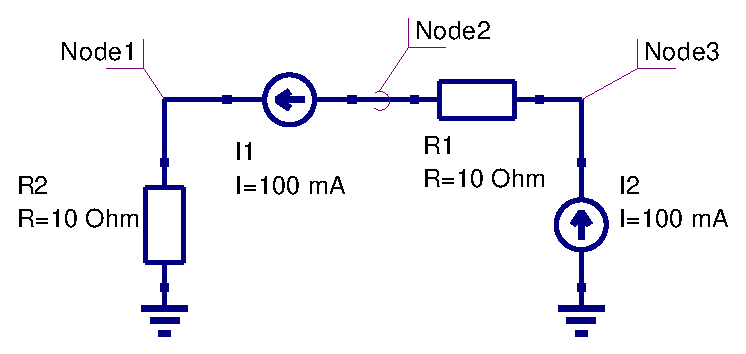
\includegraphics[width=10cm]{MNAsingular}
\end{center}
\caption{circuit with singular modified nodal analysis matrix}
\label{fig:MNAsingular}
\end{figure}
\FloatBarrier

The circuit in fig. \ref{fig:MNAsingular} has the following MNA
representation:
\begin{equation}
A x =
\begin{bmatrix}
\frac{1}{R_{2}} & 0 & 0\\
0 & \frac{1}{R_{1}} & -\frac{1}{R_{1}}\\
0 & -\frac{1}{R_{1}} & \frac{1}{R_{1}}
\end{bmatrix}
\cdot
\begin{bmatrix}
V_1\\
V_2\\
V_3
\end{bmatrix}
=
\begin{bmatrix}
0.1 & 0 & 0\\
0 & 0.1 & -0.1\\
0 & -0.1 & 0.1
\end{bmatrix}
\cdot
\begin{bmatrix}
V_1\\
V_2\\
V_3
\end{bmatrix}
=
\begin{bmatrix}
I_1\\
-I_1\\
I_2
\end{bmatrix}
=
\begin{bmatrix}
0.1\\
-0.1\\
0.1
\end{bmatrix}
=
z
\end{equation}

The second and third row of the matrix $A$ are linear dependent and
the matrix is singular because its determinant is zero.  Depending on
the right hand side $z$, the equation system has none or unlimited
solutions.  This is called an under-determined system.  The discussed
QR decomposition easily computes a valid solution without reducing
accuracy.  The LU decomposition would probably fail because of the
singularity.

\subsubsection{QR decomposition with column pivoting}
%\addcontentsline{toc}{subsubsection}{QR decomposition with column pivoting}

\subsubsection{Least norm problem}
%\addcontentsline{toc}{subsubsection}{Least norm problem}

With some more effort it is possible to obtain the minimum-norm
solution of this problem.  The algorithm as described here would
probably yield the following solution:
\begin{equation}
x =
\begin{bmatrix}
V_1\\
V_2\\
V_3
\end{bmatrix}
=
\begin{bmatrix}
1\\
0\\
1
\end{bmatrix}
\end{equation}

This is one out of unlimited solutions.  The following short
description shows how it is possible to obtain the minimum-norm
solution.  When decomposing the transposed problem
\begin{equation}
A^T = Q\cdot R
\end{equation}

the minimum-norm solution $\hat{x}$ is obtained by forward substitution of
\begin{equation}
R^T\cdot x = z
\end{equation}

and multiplying the result with $Q$.
\begin{equation}
\hat{x} = Q\cdot x
\end{equation}

In the example above this algorithm results in a solution vector with
the least vector norm possible:
\begin{equation}
\hat{x} =
\begin{bmatrix}
V_1\\
V_2\\
V_3
\end{bmatrix}
=
\begin{bmatrix}
1\\
-0.5\\
0.5
\end{bmatrix}
\end{equation}

This algorithm outline is also sometimes called LQ decomposition
because of $R^T$ being a lower triangular matrix used by the forward
substitution.

\subsection{Singular value decomposition}
%\addcontentsline{toc}{subsection}{Singular value decomposition}

Very bad conditioned (ratio between largest and smallest eigenvalue)
matrices, i.e. nearly singular, or even singular matrices (over- or
under-determined equation systems) can be handled by the singular
value decomposition (SVD).  This type of decomposition is defined by
\begin{equation}
\label{eq:USV}
A = U\cdot \Sigma\cdot V^H
\end{equation}

where the $U$ matrix consists of the orthonormalized eigenvectors
associated with the eigenvalues of $A\cdot A^H$, $V$ consists of the
orthonormalized eigenvectors of $A^H\cdot A$ and $\Sigma$ is a matrix
with the singular values of $A$ (non-negative square roots of the
eigenvalues of $A^H\cdot A$) on its diagonal and zeros otherwise.
\begin{equation}
\Sigma =
\begin{bmatrix}
\sigma_1 & 0 & \cdots & 0\\
0 & \sigma_2 & \cdots & 0\\
\vdots & \vdots & \ddots & \vdots\\
0 & 0 & \cdots & \sigma_n
\end{bmatrix}
\end{equation}

The singular value decomposition can be used to solve linear equation
systems by simple substitutions
\begin{align}
A\cdot x &= z\\
U\cdot \Sigma\cdot V^H\cdot x &= z\\
\Sigma\cdot V^H\cdot x &= U^H\cdot z
\end{align}
since
\begin{equation}
U^H\cdot U = V^H\cdot V = V\cdot V^H = I
\end{equation}

To obtain the decomposition stated in eq.~\eqref{eq:USV} Householder
vectors are computed and their transformations are applied from the
left-hand side and right-hand side to obtain an upper bidiagonal
matrix $B$ which has the same singular values as the original $A$
matrix because all of the transformations introduced are orthogonal.
\begin{equation}
U_B^{H\,(n)}\cdot\ldots\cdot U_B^{H\,(1)}\cdot A\cdot
V_B^{(1)}\cdot\ldots\cdot V_B^{(n-2)}
= U_B^H\cdot A\cdot V_B = B^{(0)}
\end{equation}

Specifically, $U_B^{H\,(i)}$ annihilates the subdiagonal elements in
column $i$ and $V_B^{(j)}$ zeros out the appropriate elements in row
$j$.
\begin{equation}
B^{(0)} = 
\begin{bmatrix}
\beta_1 & \delta_2 & 0 & \cdots & 0\\
0 & \beta_2 & \delta_3 & 0 & 0\\
\vdots & 0 & \ddots & \ddots & 0\\
0 & 0 & 0 & \beta_{n-1} & \delta_n\\
0 & 0 & 0 & 0 & \beta_n\\
\end{bmatrix}
\end{equation}

Afterwards an iterative process (which turns out to be a QR iteration)
is used to transform the bidiagonal matrix $B$ into a diagonal form by
applying successive Givens transformations (therefore orthogonal as
well) to the bidiagonal matrix.  This iteration is said to have cubic
convergence and yields the final singular values of the matrix $A$.
\begin{equation}
B^{(0)} \rightarrow B^{(1)}\rightarrow \ldots \rightarrow \Sigma
\end{equation}
\begin{equation}
B^{(k+1)} = \left(\tilde{U}^{(k)}\right)^H\cdot B^{(k)}\cdot \tilde{V}^{(k)}
\end{equation}

Each of the transformations applied to the bidiagonal matrix is also
applied to the matrices $U_B$ and $V_B^H$ which finally yield the $U$
and $V^H$ matrices after convergence.

\addvspace{12pt}

So far for the algorithm outline.  Without the very details the
following sections briefly describe each part of the singular value
decomposition.

\subsubsection{Notation}

Beforehand some notation marks are going to be defined.

\begin{itemize}

\item Conjugate transposed (or adjoint):
\begin{equation*}
A \rightarrow \left(A^T\right)^* = \left(A^*\right)^T = A^H
\end{equation*}


\item Euclidean norm:
\begin{equation*}
\lVert x \rVert = \sqrt{\sum^n_{i=1} x_i\cdot x^*_1} =
\sqrt{\sum^n_{i=1} \lvert x_i\rvert^2} = 
\sqrt{\lvert x_1\rvert^2 + \cdots  + \lvert x_n\rvert^2} = 
\sqrt{x\cdot x^H}
\end{equation*}

\item Hermitian (or self adjoint):
\begin{equation*}
A = A^H
\end{equation*}
whereas $A^H$ denotes the conjugate transposed matrix of $A$.  In the
real case the matrix $A$ is then said to be ``symmetric''.

\item Unitary:
\begin{equation*}
A\cdot A^H = A^H\cdot A = I
\end{equation*}
Real matrices $A$ with this property are called ``orthogonal''.

\end{itemize}

\subsubsection{Householder reflector}

A Householder matrix is an elementary unitary matrix that is
Hermitian.  Its fundamental use is their ability to transform a vector
$x$ to a multiple of $\vec{e}_1$, the first column of the identity
matrix.  The elementary Hermitian (i.e. the Householder matrix) is
defined as
\begin{equation}
H = I - 2\cdot u\cdot u^H
\;\;\;\;
\textrm{ where }
\;\;\;\;
u^H\cdot u = 1
\end{equation}

Beside excellent numerical properties, their application demonstrates
their efficiency.  If $A$ is a matrix, then
\begin{align}
H\cdot A &= A - 2\cdot u\cdot u^H\cdot A\\
\nonumber
&=  A - 2\cdot u\cdot \left(A^H\cdot u\right)^H
\end{align}
and hence explicit formation and storage of $H$ is not required.  Also
columns (or rows) can be transformed individually exploiting the fact
that $u^H\cdot A$ yields a scalar product for single columns or rows.

\paragraph{Specific case}

In order to reduce a 4$\times$4 matrix $A$ to upper triangular form
successive Householder reflectors must be applied.
\begin{equation}
A =
\begin{bmatrix}
a_{11} & a_{12} & a_{13} & a_{14}\\
a_{21} & a_{22} & a_{23} & a_{24}\\
a_{31} & a_{32} & a_{33} & a_{34}\\
a_{41} & a_{42} & a_{43} & a_{44}
\end{bmatrix}
\end{equation}

In the first step the diagonal element $a_{11}$ gets replaced and its
below elements get annihilated by the multiplication with an
appropriate Householder vector, also the remaining right-hand columns
get modified.
\begin{equation}
u_1 =
\begin{bmatrix}
u_{11}\\
u_{21}\\
u_{31}\\
u_{41}
\end{bmatrix}
\;\;\;\;
H_1 = I - 2\cdot u_1\cdot u_1^H
\;\;\;\;
\rightarrow A_1 = H_1\cdot A =
\begin{bmatrix}
\beta_1 & a_{12}^{(1)} & a_{13}^{(1)} & a_{14}^{(1)}\\
0 & a_{22}^{(1)} & a_{23}^{(1)} & a_{24}^{(1)}\\
0 & a_{32}^{(1)} & a_{33}^{(1)} & a_{34}^{(1)}\\
0 & a_{42}^{(1)} & a_{43}^{(1)} & a_{44}^{(1)}
\end{bmatrix}
\end{equation}

This process must be repeated
\begin{equation}
u_2 =
\begin{bmatrix}
0\\
u_{22}\\
u_{32}\\
u_{42}
\end{bmatrix}
\;\;\;\;
H_2 = I - 2\cdot u_2\cdot u_2^H
\;\;\;\;
\rightarrow A_2 = H_2\cdot A_1 =
\begin{bmatrix}
\beta_1 & a_{12}^{(2)} & a_{13}^{(2)} & a_{14}^{(2)}\\
0 & \beta_2 & a_{23}^{(2)} & a_{24}^{(2)}\\
0 & 0 & a_{33}^{(2)} & a_{34}^{(2)}\\
0 & 0 & a_{43}^{(2)} & a_{44}^{(2)}
\end{bmatrix}
\end{equation}

\begin{equation}
u_3 =
\begin{bmatrix}
0\\
0\\
u_{33}\\
u_{43}
\end{bmatrix}
\;\;\;\;
H_3 = I - 2\cdot u_3\cdot u_3^H
\;\;\;\;
\rightarrow A_3 = H_3\cdot A_2 =
\begin{bmatrix}
\beta_1 & a_{12}^{(3)} & a_{13}^{(3)} & a_{14}^{(3)}\\
0 & \beta_2 & a_{23}^{(3)} & a_{24}^{(3)}\\
0 & 0 & \beta_3 & a_{34}^{(3)}\\
0 & 0 & 0 & a_{44}^{(3)}
\end{bmatrix}
\end{equation}

\begin{equation}
u_4 =
\begin{bmatrix}
0\\
0\\
0\\
u_{44}
\end{bmatrix}
\;\;\;\;
H_4 = I - 2\cdot u_4\cdot u_4^H
\;\;\;\;
\rightarrow A_4 = H_4\cdot A_3 =
\begin{bmatrix}
\beta_1 & a_{12}^{(4)} & a_{13}^{(4)} & a_{14}^{(4)}\\
0 & \beta_2 & a_{23}^{(4)} & a_{24}^{(4)}\\
0 & 0 & \beta_3 & a_{34}^{(4)}\\
0 & 0 & 0 & \beta_4
\end{bmatrix}
\end{equation}

until the matrix $A$ contains an upper triangular matrix $R$.  The
matrix $Q$ can be expressed as the the product of the Householder
vectors.  The performed operations deliver
\begin{equation}
H^H_4\cdot H^H_3\cdot H^H_2\cdot H^H_1 \cdot A = Q^H\cdot A = R
\;\;\;\; \rightarrow \;\;\;\;
A = Q\cdot R
\end{equation}

since $Q$ is unitary.  The matrix $Q$ itself can be expressed in terms
of $H_i$ using the following transformation.
\begin{align}
\label{eq:qh_1}
Q^H &= H^H_4\cdot H^H_3\cdot H^H_2\cdot H^H_1\\
\left(Q^H\right)^H &= \left(H^H_4\cdot H^H_3\cdot H^H_2\cdot H^H_1\right)^H\\
\label{eq:qh_3}
Q &= H_1\cdot H_2\cdot H_3\cdot H_4
\end{align}

The eqn.~\eqref{eq:qh_1}-\eqref{eq:qh_3} are necessary to be mentioned
only in case $Q$ is not Hermitian, but still unitary.  Otherwise there
is no difference computing $Q$ or $Q^H$ using the Householder vectors.
No care must be taken in choosing forward or backward accumulation.

\paragraph{General case}

In the general case it is necessary to find an elementary unitary
matrix
\begin{equation}
H = I - \tau\cdot u\cdot u^H
\end{equation}
that satisfies the following three conditions.
\begin{equation}
\label{eq:herm_cond}
\left|\tau\right|^2\cdot u^H\cdot u = \tau + \tau^* =
2\cdot Re\left\{\tau \right\}
\;\;\;\; , \;\;\;\;
H^H\cdot x = \gamma\cdot \lVert x \rVert \cdot \vec{e}_1
\;\;\;\; , \;\;\;\;
\lvert \gamma \rvert = 1
\end{equation}

When choosing the elements $u_{ii} = 1$ it is possible the store the
Householder vectors as well as the upper triangular matrix $R$ in the
same storage of the matrix $A$.  The Householder matrices $H_i$ can be
completely restored from the Householder vectors.
\begin{equation}
A =
\begin{bmatrix}
\beta_1 & a_{12} & a_{13} & a_{14}\\
u_{21} & \beta_2 & a_{23} & a_{24}\\
u_{31} & u_{32} & \beta_3 & a_{34}\\
u_{41} & u_{42} & u_{43} & \beta_4
\end{bmatrix}
\end{equation}

There exist several approaches to meet the conditions expressed in
eq. \eqref{eq:herm_cond}.  For fewer computational effort it may be
convenient to choose $\gamma$ to be real valued.  With the notation
\begin{equation}
H^H\cdot x =
H^H\cdot
\begin{bmatrix}
\alpha\\
x_2\\
x_3\\
x_4\\
\end{bmatrix}
=
\begin{bmatrix}
\beta\\
0\\
0\\
0\\
\end{bmatrix}
\end{equation}

one possibility is to define the following calculation rules.
\begin{align}
\nu &= sign\left(Re\left\{\alpha\right\}\right)\cdot \lVert x \rVert\\
\tau &= \dfrac{\alpha + \nu}{\nu}\\
\gamma &= -1\\
\beta &= \gamma \cdot \lVert x \rVert = - \lVert x \rVert
\;\;\;\; \rightarrow \;\;\;\;
\textrm{real valued}\\
u &= \dfrac{x + \nu\cdot \vec{e}_1}{\alpha + \nu}
\;\;\;\; \rightarrow \;\;\;\;
u_{ii} = 1
\end{align}

These definitions yield a complex $\tau$, thus $H$ is no more
Hermitian but still unitary.
\begin{equation}
H = I - \tau\cdot u\cdot u^H
\;\;\;\; \rightarrow \;\;\;\;
H^H = I - \tau^*\cdot u\cdot u^H
\end{equation}

\subsubsection{Givens rotation}

A Givens rotation is a plane rotation matrix.  Such a plane rotation
matrix is an orthogonal matrix that is different from the identity
matrix only in four elements.
\begin{equation}
\label{eq:rotation}
M =
\left[
\begin{array}{ccccccccccc}
1 & 0 & \cdots &  &  &  &  &  &  & \cdots & 0\\
0 & \ddots &  &  &  &  &  &  &  &  & \vdots\\
\vdots &  & 1 &  &  &  &  &  &  &  & \\
 &  &  & +c & 0 & \cdots & 0 & +s &  &  & \\
 &  &  & 0 & 1 &  &  & 0 &  &  & \\
 &  &  & \vdots &  & \ddots &  & \vdots &  &  & \\
 &  &  & 0 &  &  & 1 & 0 &  &  & \\
 &  &  & -s & 0 & \cdots & 0 & +c &  &  & \\
 &  &  &  &  &  &  &  & 1 &  & \vdots\\
\vdots &  &  &  &  &  &  &  &  & \ddots & 0\\
0 & \cdots &  &  &  &  &  &  & \cdots & 0 & 1
\end{array}
\right]
\end{equation}

The elements are usually chosen so that
\begin{equation}
\label{eq:givenscond}
R =
\left[\begin{array}{rl}
c & s\\
-s & c\\
\end{array}\right]
\;\;\;\;  \;\;\;\;
c = \cos{\theta},\; s = \sin{\theta}
\;\;\;\; \rightarrow \;\;\;\;
\left|c\right|^2 + \left|s\right|^2 = 1
\end{equation}

The most common use of such a plane rotation is to choose $c$ and $s$
such that for a given $a$ and $b$
\begin{equation}
\label{eq:givensrot}
R =
\left[\begin{array}{rl}
c & s\\
-s & c\\
\end{array}\right]
\cdot
\begin{bmatrix}
a\\
b\\
\end{bmatrix}
=
\begin{bmatrix}
d\\
0\\
\end{bmatrix}
\end{equation}
multiplication annihilates the lower vector entry.  In such an
application the matrix $R$ is often termed ``Givens rotation'' matrix.
The following equations satisfy eq.~\eqref{eq:givensrot} for a given
$a$ and $b$ exploiting the conditions given in
eq.~\eqref{eq:givenscond}.
\begin{equation}
c = \dfrac{\pm a}{\sqrt{\left|a\right|^2 + \left|b\right|^2}}
\;\;\;\; \textrm{and} \;\;\;\;
s = \dfrac{\pm b}{\sqrt{\left|a\right|^2 + \left|b\right|^2}}
\end{equation}
\begin{equation}
d = \sqrt{\left|a\right|^2 + \left|b\right|^2}
\end{equation}

\subsubsection{Eigenvalues of a 2-by-2 matrix}

The eigenvalues of a 2-by-2 matrix
\begin{equation}
A = 
\begin{bmatrix}
a & b\\
c & d
\end{bmatrix}
\end{equation}

can be obtained directly from the quadratic formula.  The
characteristic polynomial is
\begin{equation}
\begin{split}
det\left(A -\mu I\right) =
det 
\begin{bmatrix}
a - \mu & b\\
c & d - \mu
\end{bmatrix}
&= \left(a -\mu\right) \cdot \left(d -\mu\right) - bc\\
0 &= \mu^2 - \left(a + d\right)\cdot\mu + \left(ad - bc\right)
\end{split}
\end{equation}

The polynomial yields the two eigenvalues.
\begin{equation}
\label{eq:eigenvalue}
\mu_{1,2} = \dfrac{a + d}{2} \pm \sqrt{\left(\dfrac{a + d}{2}\right)^2 + bc - ad}
\end{equation}

For a symmetric matrix $A$ (i.e. $b = c$) eq.\eqref{eq:eigenvalue} can
be rewritten to:
\begin{equation}
\label{eq:eigenvalue_sym}
\mu_{1,2} = e + d  \pm \sqrt{e^2 + b^2}
\;\;\;\; \textrm{ with } \;\;\;\;
e = \dfrac{a - d}{2}
\end{equation}

\subsubsection{Step 1: Bidiagonalization}

In the first step the original matrix $A$ is bidiagonalized by the
application of Householder reflections from the left and right hand
side.  The matrices $U_B^H$ and $V_B$ can each be determined as a
product of Householder matrices.
\begin{equation}
\underbrace{U_B^{H\,(n)}\cdot\ldots\cdot U_B^{H\,(1)}}_{U_B^H}\cdot A\cdot
\underbrace{V_B^{(1)}\cdot\ldots\cdot V_B^{(n-2)}}_{V_B}
= U_B^H\cdot A\cdot V_B = B^{(0)}
\end{equation}

Each of the required Householder vectors are created and applied as
previously defined.  Suppose a $n\times n$ matrix, then applying the
first Householder vector from the left hand side eliminates the first
column and yields
\begin{align}
U_B^{H\,(1)} \cdot A &=
\begin{bmatrix}
\boldsymbol{\beta_1} & a_{12}^{(1)} & a_{13}^{(1)} & \cdots & a_{1n}^{(1)} \\
u_{21} & a_{22}^{(1)} & a_{23}^{(1)} &  & a_{2n}^{(1)} \\
u_{31} & a_{32}^{(1)} & a_{33}^{(1)} &  & a_{3n}^{(1)} \\
\vdots &  & & \ddots & \vdots \\
u_{n1} & a_{n2}^{(1)} & a_{n3}^{(1)} & \cdots & a_{nn}^{(1)} \\
\end{bmatrix}\\
%\end{align}
\intertext{
Next, a Householder vector is applied from the right hand side to
annihilate the first row.
}
%\begin{align}
U_B^{H\,(1)} \cdot A \cdot V_B^{(1)} &=
\begin{bmatrix}
\beta_1 & \boldsymbol{\delta_2} & v_{13} & \cdots & v_{1n} \\
u_{21} & a_{22}^{(2)} & a_{23}^{(2)} &  & a_{2n}^{(2)} \\
u_{31} & a_{32}^{(2)} & a_{33}^{(2)} &  & a_{3n}^{(2)} \\
\vdots &  & & \ddots & \vdots \\
u_{n1} & a_{n2}^{(2)} & a_{n3}^{(2)} & \cdots & a_{nn}^{(2)} \\
\end{bmatrix}\\
%\end{align}
\intertext{
Again, a Householder vector is applied from the left hand side to
annihilate the second column.
}
%\begin{align}
U_B^{H\,(2)} \cdot U_B^{H\,(1)} \cdot A \cdot V_B^{(1)} &=
\begin{bmatrix}
\beta_1 & \delta_2 & v_{13} & \cdots & v_{1n} \\
u_{21} & \boldsymbol{\beta_2} & a_{23}^{(3)} &  & a_{2n}^{(3)} \\
u_{31} & u_{32} & a_{33}^{(3)} &  & a_{3n}^{(3)} \\
\vdots & \vdots & & \ddots & \vdots \\
u_{n1} & u_{n2} & a_{n3}^{(3)} & \cdots & a_{nn}^{(3)} \\
\end{bmatrix}\\
%\end{align}
\intertext{
This process is continued until
}
%\begin{align}
U_B^H \cdot A \cdot V_B &=
\begin{bmatrix}
\beta_1 & \delta_2 & v_{13} & \cdots & v_{1n} \\
u_{21} & \beta_2 & \delta_3 &  & v_{2n} \\
u_{31} & u_{32} & \ddots & \ddots &  \\
\vdots & \vdots & & \beta_{n-1} & \delta_n \\
u_{n1} & u_{n2} & u_{n3} &  & \boldsymbol{\beta_n} \\
\end{bmatrix}
\end{align}

For each of the Householder transformations from the left and right
hand side the appropriate $\tau$ values must be stored in separate
vectors.

\subsubsection{Step 2: Matrix reconstructions}

Using the Householder vectors stored in place of the original $A$
matrix and the appropriate $\tau$ value vectors it is now necessary to
unpack the $U_B$ and $V_B^H$ matrices.  The diagonal vector $\beta$
and the super-diagonal vector $\delta$ can be saved in separate
vectors previously.  Thus the $U_B$ matrix can be unpacked in place of
the $A$ matrix and the $V_B^H$ matrix is unpacked in a separate
matrix.

\addvspace{12pt}

There are two possible algorithms for computing the Householder
product matrices, i.e. forward accumulation and backward accumulation.
Both start with the identity matrix which is successively multiplied
by the Householder matrices either from the left or right.
\begin{align}
U_B^H &= H^H_{Un}\cdot \ldots \cdot H^H_{U2}\cdot H^H_{U1}\cdot I\\
\rightarrow\;\;\;\; U_B\; &= I\cdot H_{Un}\cdot \ldots \cdot H_{U2}\cdot H_{U1}
\end{align}

Recall that the leading portion of each Householder matrix is the
identity except the first.  Thus, at the beginning of backward
accumulation, $U_B$ is ``mostly the identity'' and it gradually
becomes full as the iteration progresses.  This pattern can be
exploited to reduce the number of required flops.  In contrast,
$U_B^H$ is full in forward accumulation after the first step.  For
this reason, backward accumulation is cheaper and the strategy of
choice.  When unpacking the $U_B$ matrix in place of the original $A$
matrix it is necessary to choose backward accumulation anyway.
\begin{align}
V_B\; &= I\cdot H^H_{V1}\cdot H^H_{V2}\cdot \ldots \cdot H^H_{Vn}\\
\rightarrow\;\;\;\; V_B^H &= I\cdot H_{Vn}\cdot \ldots \cdot H_{V2}\cdot H_{V1}
\end{align}

Unpacking the $V_B^H$ matrix is done in a similar way also performing
successive Householder matrix multiplications using backward
accumulation.

\subsubsection{Step 3: Diagonalization -- shifted QR iteration}

At this stage the matrices $U_B$ and $V_B^H$ exist in unfactored form.
Also there are the diagonal vector $\beta$ and the super-diagonal
vector $\delta$.  Both vectors are real valued.  Thus the following
algorithm can be applied even though solving a complex equation
system.
\begin{equation}
B^{(0)} = 
\begin{bmatrix}
\beta_1 & \delta_2 & 0 & \cdots & 0\\
0 & \beta_2 & \delta_3 & 0 & 0\\
\vdots & 0 & \ddots & \ddots & 0\\
0 & 0 & 0 & \beta_{n-1} & \delta_n\\
0 & 0 & 0 & 0 & \beta_n\\
\end{bmatrix}
\end{equation}

The remaining problem is thus to compute the SVD of the matrix $B$.
This is done applying an implicit-shift QR step to the tridiagonal
matrix $T=B^T B$ which is a symmetric.  The matrix $T$ is not
explicitly formed that is why a QR iteration with implicit shifts is
applied.

\addvspace{12pt}

After bidiagonalization we have a bidiagonal matrix $B^{(0)}$:
\begin{equation}
B^{(0)} = U_B^H \cdot A \cdot V_B
\end{equation}

The presented method turns $B^{(k)}$ into a matrix $B^{(k+1)}$ by
applying a set of orthogonal transforms
\begin{equation}
\label{eq:svd_step}
B^{(k+1)} = \tilde{U}^H\cdot B^{(k)} \cdot \tilde{V}
\end{equation}

The orthogonal matrices $\tilde{U}$ and $\tilde{V}$ are chosen so that
$B^{(k+1)}$ is also a bidiagonal matrix, but with the super-diagonal
elements smaller than those of $B^{(k)}$.  The eq.\eqref{eq:svd_step}
is repeated until the non-diagonal elements of $B^{(k+1)}$ become
smaller than $\varepsilon$ and can be disregarded.

\addvspace{12pt}

The matrices $\tilde{U}$ and $\tilde{V}$ are constructed as
\begin{equation}
\tilde{U} = \tilde{U}_1 \cdot \tilde{U}_2 \cdot \tilde{U}_3\cdot \dots \cdot \tilde{U}_{n-1}
\end{equation}

and similarly $\tilde{V}$ where $\tilde{V}_i$ and $\tilde{U}_i$ are
matrices of simple rotations as given in eq.\eqref{eq:rotation}.  Both
$\tilde{V}$ and $\tilde{U}$ are products of Givens rotations and thus
perform orthogonal transforms.

\paragraph{Single shifted QR step.}

The left multiplication of $B^{(k)}$ by $\tilde{U}_i^H$ replaces two
rows of $B^{(k)}$ by their linear combinations.  The rest of $B^{(k)}$
is unaffected.  Right multiplication of $B^{(k)}$ by $\tilde{V}_i$
similarly changes only two columns of $B^{(k)}$.

\addvspace{12pt}

A matrix $\tilde{V}_1$ is chosen the way that
\begin{equation}
B^{(k)}_1 = B^{(k)}_0 \cdot \tilde{V}_1
\end{equation}
 
is a QR transform with a shift.  Note that multiplying $B^{(k)}$ by
$\tilde{V}_1$ gives rise to a non-zero element which is below the main
diagonal.
\begin{equation}
B^{(k)}_0 \cdot \tilde{V}_1 =
\begin{bmatrix}
\times & \times & 0 & 0 & 0 & 0\\
\framebox{$\otimes$} & \times & \times & 0 & 0 & 0\\
0 & 0 & \times & \times & 0 & 0\\
0 & 0 & 0 & \times & \times & 0\\
0 & 0 & 0 & 0 & \times & \times\\
0 & 0 & 0 & 0  & 0 & \times\\
\end{bmatrix}
\end{equation}

A new rotation angle is then chosen so that multiplication by
$\tilde{U}_1^H$ gets rid of that element.  But this will create a
non-zero element which is right beside the super-diagonal.
\begin{equation}
\tilde{U}_1^H \cdot B^{(k)}_1 =
\begin{bmatrix}
\times & \times & \framebox{$\otimes$} & 0 & 0 & 0\\
0 & \times & \times & 0 & 0 & 0\\
0 & 0 & \times & \times & 0 & 0\\
0 & 0 & 0 & \times & \times & 0\\
0 & 0 & 0 & 0 & \times & \times\\
0 & 0 & 0 & 0  & 0 & \times\\
\end{bmatrix}
\end{equation}

Then $\tilde{V}_2$ is made to make it disappear, but this leads to
another non-zero element below the diagonal, etc.
\begin{equation}
B^{(k)}_2 \cdot \tilde{V}_2 =
\begin{bmatrix}
\times & \times & 0 & 0 & 0 & 0\\
0 & \times & \times & 0 & 0 & 0\\
0 & \framebox{$\otimes$} & \times & \times & 0 & 0\\
0 & 0 & 0 & \times & \times & 0\\
0 & 0 & 0 & 0 & \times & \times\\
0 & 0 & 0 & 0  & 0 & \times\\
\end{bmatrix}
\end{equation}

In the end, the matrix $\tilde{U}^H B \tilde{V}$ becomes bidiagonal
again.  However, because of a special choice of $\tilde{V}_1$ (QR
algorithm), its non-diagonal elements are smaller than those of $B$.

\addvspace{12pt}

Please note that each of the transforms must also be applied to the
unfactored $U_B^H$ and $V_B$ matrices which turns them successively
into $U^H$ and $V$

\paragraph{Computation of the Wilkinson shift.}

For a single QR step the computation of the eigenvalue $\mu$ of the
trailing 2-by-2 submatrix of $T_n = B_n^T\cdot B_n$ that is closer to
the $t_{22}$ matrix element is required.
\begin{align}
T_n =
\begin{bmatrix}
t_{11} & t_{12}\\
t_{21} & t_{22}\\
\end{bmatrix}
= B_n^T\cdot B_n &=
\begin{bmatrix}
\delta_{n-1} & \beta_{n-1} & 0\\
0 & \delta_{n} & \beta_{n}\\
\end{bmatrix} \cdot
\begin{bmatrix}
\delta_{n-1} & 0\\
\beta_{n-1} & \delta_{n}\\
0 & \beta_{n}\\
\end{bmatrix}\\
&=
\begin{bmatrix}
\beta_{n-1}^2 + \delta_{n-1}^2 & \delta_{n}\cdot \beta_{n-1}\\
\delta_{n}\cdot \beta_{n-1} & \beta_{n}^2 + \delta_{n}^2\\
\end{bmatrix}
\end{align}

The required eigenvalue is called Wilkinson shift, see
eq.\eqref{eq:eigenvalue_sym} for details.  The sign for the eigenvalue
is chosen such that it is closer to $t_{22}$.
\begin{align}
\mu &= t_{22} + d - sign(d)\cdot \sqrt{d^2 + t_{12}^2}\\
&= t_{22} + d - t_{12}\cdot sign\left(\dfrac{d}{t_{12}}\right)\cdot \sqrt{\left(\dfrac{d}{t_{12}}\right)^2 + 1}\\
&= t_{22} - \dfrac{t_{12}^2}{d + t_{12}\cdot sign\left(\dfrac{d}{t_{12}}\right)\cdot \sqrt{\left(\dfrac{d}{t_{12}}\right)^2 + 1}}
\end{align}
whereas
\begin{equation}
d = \dfrac{t_{11} - t_{22}}{2}
\end{equation}

The Givens rotation $\tilde{V}_1$ is chosen such that
\begin{equation}
\begin{bmatrix}
c_1 & s_1\\
-s_1 & c_1\\
\end{bmatrix}^T
\cdot
\begin{bmatrix}
(\beta_1^2 - \mu) / \beta_1 \\
\delta_2
\end{bmatrix}
=
\begin{bmatrix}
\times\\
0
\end{bmatrix}
\end{equation}

The special choice of this first rotation in the single QR step
ensures that the super-diagonal matrix entries get smaller.
Typically, after a few of these QR steps, the super-diagonal entry
$\delta_n$ becomes negligible.

\paragraph{Zeros on the diagonal or super-diagonal.}

The QR iteration described above claims to hold if the underlying
bidiagonal matrix is unreduced, i.e. has no zeros neither on the
diagonal nor on the super-diagonal.

\addvspace{12pt}

When there is a zero along the diagonal, then premultiplication by a
sequence of Givens transformations can zero the right-hand
super-diagonal entry as well.  The inverse rotations must be applied
to the $U_B^H$ matrix.
\begin{align*}
B = &
\begin{bmatrix}
\times & \times & 0 & 0 & 0 & 0\\
0 & \times & \times & 0 & 0 & 0\\
0 & 0 & 0 & \times & 0 & 0\\
0 & 0 & 0 & \times & \times & 0\\
0 & 0 & 0 & 0 & \times & \times\\
0 & 0 & 0 & 0  & 0 & \times\\
\end{bmatrix}
&\rightarrow  &
\begin{bmatrix}
\times & \times & 0 & 0 & 0 & 0\\
0 & \times & \times & 0 & 0 & 0\\
0 & 0 & 0 & 0 & \otimes & 0\\
0 & 0 & 0 & \times & \times & 0\\
0 & 0 & 0 & 0 & \times & \times\\
0 & 0 & 0 & 0  & 0 & \times\\
\end{bmatrix}\\
\rightarrow &
\begin{bmatrix}
\times & \times & 0 & 0 & 0 & 0\\
0 & \times & \times & 0 & 0 & 0\\
0 & 0 & 0 & 0 & 0 & \otimes\\
0 & 0 & 0 & \times & \times & 0\\
0 & 0 & 0 & 0 & \times & \times\\
0 & 0 & 0 & 0  & 0 & \times\\
\end{bmatrix}
&\rightarrow &
\begin{bmatrix}
\times & \times & 0 & 0 & 0 & 0\\
0 & \times & \times & 0 & 0 & 0\\
0 & 0 & 0 & 0 & 0 & 0\\
0 & 0 & 0 & \times & \times & 0\\
0 & 0 & 0 & 0 & \times & \times\\
0 & 0 & 0 & 0  & 0 & \times\\
\end{bmatrix}
\end{align*}

Thus the problem can be decoupled into two smaller matrices $B_1$ and
$B_2$.  The diagonal matrix $B_3$ is successively getting larger for
each super-diagonal entry being neglected after the QR iterations.
\begin{equation}
\begin{bmatrix}
B_1 & 0 & 0\\
0 & B_2 & 0\\
0 & 0 & B_3\\
\end{bmatrix}
\end{equation}

Matrix $B_2$ has non-zero super-diagonal entries.  If there is any
zero diagonal entry in $B_2$, then the super-diagonal entry can be
annihilated as just described.  Otherwise the QR iteration algorithm
can be applied to $B_2$.

\addvspace{12pt}

When there are only $B_3$ matrix entries left (diagonal entries only)
the algorithm is finished, then the $B$ matrix has been transformed
into the singular value matrix $\Sigma$.

\subsubsection{Step 4: Solving the equation system}

It is straight-forward to solve a given equation system once having
the singular value decomposition computed.
\begin{align}
A\cdot x &= z\\
U\Sigma V^H\cdot x &= z\\
\Sigma V^H\cdot x &= U^H \cdot z\\
V^H\cdot x &= \Sigma^{-1} U^H \cdot z\\
x &= V\Sigma^{-1} U^H \cdot z
\label{eq:svd_solution}
\end{align}

The inverse of the diagonal matrix $\Sigma$ yields
\begin{equation}
\Sigma^{-1} =
\begin{bmatrix}
1/\sigma_1 & 0 & \cdots & 0\\
0 & 1/\sigma_2 & \cdots & 0\\
\vdots & \vdots & \ddots & \vdots\\
0 & 0 & \cdots & 1/\sigma_n
\end{bmatrix}
\end{equation}

With $v_i$ being the i-th row of the matrix $V$, $u_i$ the i-th column
of the matrix $U$ and $\sigma_i$ the i-th singular value
eq.~\eqref{eq:svd_solution} can be rewritten to
\begin{equation}
x = \sum_{i=1}^{n} \dfrac{u_i^H\cdot z}{\sigma_i}\cdot v_i
\end{equation}

It must be mentioned that very small singular values $\sigma_i$
corrupt the complete result.  Such values indicate (nearly) singular
(ill-conditioned) matrices $A$.  In such cases, the solution vector
$x$ obtained by zeroing the small $\sigma_i$'s and then using equation
\eqref{eq:svd_solution} is better than direct-method solutions (such
as LU decomposition or Gaussian elimination) and the SVD solution
where the small $\sigma_i$'s are left non-zero. It may seem
paradoxical that this can be so, since zeroing a singular value
corresponds to throwing away one linear combination of the set of
equations that is going to be solved.  The resolution of the paradox
is that a combination of equations that is so corrupted by roundoff
error is thrown away precisely as to be at best useless; usually it is
worse than useless since it "pulls" the solution vector way off
towards infinity along some direction that is almost a nullspace
vector.

\subsection{Jacobi method}
%\addcontentsline{toc}{subsection}{Jacobi method}

This method quite simply involves rearranging each equation to make
each variable a function of the other variables.  Then make an initial
guess for each solution and iterate.  For this method it is necessary
to ensure that all the diagonal matrix elements $a_{ii}$ are non-zero.
This is given for the nodal analysis and almostly given for the
modified nodal analysis.  If the linear equation system is solvable
this can always be achieved by rows substitutions.

\addvspace{12pt}

The algorithm for performing the iteration step $k + 1$ writes as
follows.
\begin{equation}
x_{i}^{(k+1)} = \dfrac{1}{a_{ii}}\left(z_i - \sum_{j=1}^{i-1} a_{ij}x_{j}^{(k)} - \sum_{j=i+1}^{n} a_{ij}x_{j}^{(k)}\right)
\;\;\;\; \textrm{ for } i = 1, \ldots, n
\end{equation}

This has to repeated until the new solution vectors $x^{(k+1)}$
deviation from the previous one $x^{(k)}$ is sufficiently small.

\addvspace{12pt}

The initial guess has no effect on whether the iterative method
converges or not, but with a good initial guess (as possibly given in
consecutive Newton-Raphson iterations) it converges faster (if it
converges).  To ensure convergence the condition
\begin{equation}
\sum_{j = 1, j \ne i}^{n} \left|a_{ij}\right| \le \left|a_{ii}\right|
\;\;\;\; \textrm{ for } i = 1, \ldots, n
\end{equation}

and at least one case
\begin{equation}
\sum_{i = 1, i \ne j}^{n} \left|a_{ij}\right| \le \left|a_{ii}\right|
\end{equation}

must apply.  If these conditions are not met, the iterative equations
may still converge.  If these conditions are met the iterative
equations will definitely converge.

\addvspace{12pt}

Another simple approach to a convergence criteria for iterative
algorithms is the Schmidt and v. Mises criteria.
\begin{equation}
\sqrt{\sum_{i = 1}^n \sum_{j = 1, j \ne i}^n \left|\dfrac{a_{ij}}{a_{ii}}\right|^2} < 1
\end{equation}

\subsection{Gauss-Seidel method}
%\addcontentsline{toc}{subsection}{Gauss-Seidel method}

The Gauss-Seidel algorithm is a modification of the Jacobi method.  It
uses the previously computed values in the solution vector of the same
iteration step.  That is why this iterative method is expected to
converge faster than the Jacobi method.

\addvspace{12pt}

The slightly modified algorithm for performing the $k + 1$ iteration
step writes as follows.
\begin{equation}
x_{i}^{(k+1)} = \dfrac{1}{a_{ii}}\left(z_i - \sum_{j=1}^{i-1} a_{ij}x_{j}^{(k+1)} - \sum_{j=i+1}^{n} a_{ij}x_{j}^{(k)}\right)
\;\;\;\; \textrm{ for } i = 1, \ldots, n
\end{equation}

The remarks about the initial guess $x^{(0)}$ as well as the
convergence criteria noted in the section about the Jacobi method
apply to the Gauss-Seidel algorithm as well.

\subsection{A comparison}
%\addcontentsline{toc}{subsection}{A comparison}

There are direct and iterative methods (algorithms) for solving linear
equation systems.  Equation systems with large and sparse matrices
should rather be solved with iterative methods.

\addvspace{12pt}

\begin{tabular}{|p{2.2cm}|p{1.5cm}|p{1.8cm}|p{2.1cm}|p{1.7cm}|p{2.95cm}|}
\hline
\raggedright method & \raggedleft precision & \raggedleft application & 
\raggedleft programming effort & \raggedleft computing complexity & 
\parbox[t]{2.95cm}{\raggedleft notes}\\
\hline
\raggedright Laplace expansion & \raggedleft numerical errors & 
\raggedleft general & \raggedleft straight forward &
\raggedleft $n!$ & \parbox[t]{2.95cm}{\raggedleft very time consuming}\\
\hline
\raggedright Gaussian elimination & \raggedleft numerical errors & 
\raggedleft general & \raggedleft intermediate & \raggedleft $n^3/3 + n^2/2$ &
\parbox[t]{2.95cm}{\raggedleft }\\
\hline
\raggedright Gauss-Jordan & \raggedleft numerical errors & \raggedleft general & \raggedleft intermediate & \raggedleft $n^3/3 + n^2 - n/3$ & \parbox[t]{2.95cm}{\raggedleft computes the inverse besides}\\
\hline
\raggedright LU decomposition & \raggedleft numerical errors & \raggedleft general & \raggedleft intermediate & \raggedleft $n^3/3 + n^2 - n/3$ & \parbox[t]{2.95cm}{\raggedleft useful for consecutive solutions}

\addvspace{1pt}

\\
\hline
\raggedright QR decomposition & \raggedleft good & \raggedleft general & \raggedleft high & \raggedleft $2n^3 + 3n^3$ & \parbox[t]{2.95cm}{\raggedleft }\\
\hline
\raggedright Singular value decomposition & \raggedleft good & \raggedleft general & \raggedleft very high & \raggedleft $2n^3 + 4n^3$ & \parbox[t]{2.95cm}{\raggedleft ill-conditioned matrices can be handled}

\addvspace{1pt}

\\
\hline
\raggedright Jacobi & \raggedleft very good & \raggedleft diagonally dominant systems & \raggedleft easy & \raggedleft $n^2$ in each iteration step & \parbox[t]{2.95cm}{\raggedleft possibly no convergence}\\
\hline
\raggedright Gauss-Seidel & \raggedleft very good & \raggedleft diagonally dominant systems & \raggedleft easy & \raggedleft $n^2$ in each iteration step & \parbox[t]{2.95cm}{\raggedleft possibly no convergence}\\
\hline
\end{tabular}

\section{Polynomial approximations}
%\addcontentsline{toc}{section}{Polynomial approximations}

\subsection{Cubic splines}
%\addcontentsline{toc}{subsection}{Cubic splines}


\section{Frequency-Time Domain Transformation}

Any signal can completely be described in time or in frequency domain.
As both representations are equivalent, it is possible to transform them
into each other. This is done by the so-called Fourier Transformation and
the inverse Fourier Transformation, respectively:
\begin{eqnarray}
\text{Fourier Transformation:} & \qquad &
     \underline{U}(j\omega) =
     \int\limits_{-\infty}^{\infty} u(t)\cdot e^{-j\omega\cdot t} \; dt \\
\text{inverse Fourier Transformation:} & \qquad &
     u(t) = \frac{1}{2\pi} \cdot \int\limits_{-\infty}^{\infty}
            \underline{U}(j\omega)\cdot e^{j\omega\cdot t} \; d\omega
\end{eqnarray}
In digital systems the data $u(t)$ or $\underline{U}(j\omega)$,
respectively, consists of a finite number $N$ of samples $u_k$ and
$\underline{U}_n$. This leads to the discrete Fourier Transformation
(DFT) and its inverse operation (IDFT):
\begin{eqnarray}
\label{eqn:DFT}
\text{DFT:} & \qquad &
     \underline{U}_n =
     \sum_{k=0}^{N-1} u_k\cdot \exp\left( -j\cdot n\frac{2\pi\cdot k}{N} \right) \\
\label{eqn:IDFT}
\text{IDFT:} & \qquad &
     u_k = \frac{1}{N} \cdot \sum_{n=0}^{N-1}
            \underline{U}_n\cdot \exp\left( j\cdot k\frac{2\pi\cdot n}{N} \right)
\end{eqnarray}
The absolute time and frequency values do not appear anymore in the DFT.
They depend on the sample frequency $f_T$ and the number of samples $N$.
\begin{equation}
\Delta f = \frac{1}{N\cdot\Delta t} = \frac{f_T}{N}
\end{equation}
Where $\Delta t$ is distance between time samples and $\Delta f$
distance between frequency samples.

\addvspace{12pt}

With DFT the $N$ time samples are transformed into $N$ frequency samples.
This also holds if the time data are real numbers, as is always
the case in "real life": The complex frequency samples are conjugate
complex symmetrical and so equalizing the score:
\begin{equation}
\underline{U}_{N-n} = \underline{U}_n^*
\end{equation}

\addvspace{12pt}

That is, knowing the input data has no imaginary part, only half of
the Fourier data must be computed.


\subsection{Fast Fourier Transformation}

As can be seen in equation \ref{eqn:DFT} the computing time of the
DFT rises with $N^2$. This is really huge, so it is
very important to reduce the time consumption. Using a strongly
optimized algorithm, the so-called Fast Fourier Transformation (FFT),
the DFT is reduced to an $N\cdot\log_2 N$ time rise.
The following information stems from \cite{Press},
where the theoretical background is explained comprehensively.

\addvspace{12pt}

The fundamental trick of the FFT is to cut the DFT into two parts,
one with data having even indices and the other with odd indices:

\begin{eqnarray}
\underline{U}_n & = &
  \sum_{k=0}^{N-1} u_k\cdot \exp\left( -j\cdot n\frac{2\pi\cdot k}{N} \right) \\
  & = & \sum_{k=0}^{N/2-1} u_{2k}\cdot
        \exp\left( -j\cdot n\frac{2\pi\cdot 2k}{N} \right) +
        \sum_{k=0}^{N/2-1} u_{2k+1}\cdot
        \exp\left( -j\cdot n\frac{2\pi\cdot (2k+1)}{N} \right) \\
  & = & \underbrace{ \sum_{k=0}^{N/2-1} u_{2k}\cdot
        \exp\left( -j\cdot n\frac{2\pi\cdot k}{N/2} \right) }_{F_{even}} +
        W_{n,N}\cdot \underbrace{ \sum_{k=0}^{N/2-1} u_{2k+1}\cdot
        \exp\left( -j\cdot n\frac{2\pi\cdot k}{N/2} \right) }_{F_{odd}} \\
\text{with} & & W_{n,N} = \exp\left( 2\pi\cdot j\cdot \frac{n}{N} \right)
        \qquad \text{(so-called 'twiddle factor')}
\end{eqnarray}

The new formula shows no speed advantages. The important thing is that
the even as well as the odd part each is again a Fourier series. Thus
the same procedure can be repeated again and again until the equation
consists of $N$ terms. Then, each term contains only one data $u_k$
with factor $e^0=1$. This works if the number of data is a power of
two (2, 4, 8, 16, 32, ...).
So finally, the FFT method performs $\log_2 N$ times the operation
\begin{equation}
\label{eqn:FFTstep}
u_{k1,even} + W_{n,x}\cdot u_{k2,odd}
\end{equation}

to get one data of $\underline{U}_n$. This is called the
Danielson-Lanzcos algorithm.
The question now arises which data values of $u_k$
needs to be combined according to equation \eqref{eqn:FFTstep}.
The answer is quite easy. The data array must be reordered by the
bit-reversal method. This means the value at index $k_1$ is swapped
with the value at index $k_2$ where $k_2$ is obtained by mirroring
the binary number $k_1$, i.e. the most significant bit becomes the
least significant one and so on. Example for $N=8$:

\addvspace{12pt}

\begin{tabular}{ccccccccccc}
000 & $\leftrightarrow$ & 000  & \qquad\qquad &  011 & $\leftrightarrow$ & 110  & \qquad\qquad &  110 & $\leftrightarrow$ & 011 \\
001 & $\leftrightarrow$ & 100  & \qquad\qquad &  100 & $\leftrightarrow$ & 001  & \qquad\qquad &  111 & $\leftrightarrow$ & 111 \\
010 & $\leftrightarrow$ & 010  & \qquad\qquad &  101 & $\leftrightarrow$ & 101 \\
\end{tabular}

\addvspace{12pt}

Having this new indexing, the values to combine according to
equation \ref{eqn:FFTstep} are the adjacent values. So, performing
the Danielson-Lanzcos algorithm has now become very easy.

\addvspace{12pt}

Figure \ref{fig:fft} illustrates the whole FFT algorithm starting with the
input data $u_k$ and ending with one value of the output data
$\underline{U}_n$.

\begin{figure}[htb]
\begin{center}
\includegraphics[width=13cm]{fft}
\end{center}
\caption{principle of a FFT with data length 8}
\label{fig:fft}
\end{figure}
\FloatBarrier

This scheme alone gives no advantage. But it can compute all output
values within, i.e. no temporary memory is needed and the periodicity
of $W_{n,N}$ is best exploited. To understand this, let's have a look
on the first Danielson-Lanczos step in figure \ref{fig:fft}. The four
multiplications and additions have to be performed for each output
value (here 8 times!). But indeed this is not true, because $W_{n,2}$
is 2-periodical in $n$ and furthermore $W_{n,2} = -W_{n+1,2}$. So now,
$u_0 + W_{0,2}\cdot u_4$ replaces the old $u_0$ value and
$u_0 - W_{0,2}\cdot u_4$ replaces the old $u_4$ value. Doing this for
all values, four multiplications and eight additions were performed
in order to calculate the first Danielson-Lanczos step for all (!!!)
output values. This goes on, as $W_{n,4}$ is 4-periodical in $n$ and
$W_{n,4} = -W_{n+2,4}$. So this time, two loop iterations (for $W_{n,4}$
and for $W_{n+1,4}$) are necessary to compute the current
Danielson-Lanczos step for all output values. This concept continues
until the last step.

\addvspace{12pt}

Finally, a complete FFT source code in C should be presented. The original
version was taken from \cite{Press}. It is a radix-2 algorithm,
known as the Cooley-Tukey Algorithm. Here, several changes were made
that gain about 10\% speed improvement.

\addvspace{12pt}

\begin{lstlisting}[language=C++,
    caption={1D-FFT algorithm in C},
    numbers=left,
    basicstyle=\small,
    frame=single,
    fontadjust]
// **************************************************************
// Parameters:
// num    - number of complex samples
// data[] - array containing the data samples, real and imaginary
//          part in alternating order (length: 2*num)
// isign  - is 1 to calculate FFT and -1 to calculate inverse FFT
// **************************************************************

#define SWAP(a,b) { wr = a; a = b; b = wr; }

void fft_radix2(int num, double *data, int isign)
{
  double wt, theta, wr, wi, wpr, wpi, tempi, tempr;
  int i, j, m, n;
  n = 2*num;
  j = 0;

  // bit reversal method
  // 1) index 0 need not to be swapped
  //    -> start at i=2
  // 2) swap scheme is symmetrical
  //    -> swap first and second half in one iteration
  for (i=2; i<num; i+=2) {
    m = num;
    while (j >= m) {  // calculate swap index
      j -= m;
      m >>= 1;
    }
    j += m;

    if(j > i) {   // was index already swapped ?
      SWAP(data[j], data[i]);     // swap real part
      SWAP(data[j+1], data[i+1]); // swap imaginary part

      if(j < num) {  // swap second half ?
        SWAP (data[n-j-2], data[n-i-2]); // swap real part
        SWAP (data[n-j-1], data[n-i-1]); // swap imaginary part
      }
    }
  }

  // Danielson-Lanzcos algorithm
  int mmax, istep;
  mmax = 2;
  while (n > mmax) { // each Danielson-Lanzcos step
    istep = mmax << 1;
    theta = isign * (2.0 * PI / mmax);
    wpr = cos(theta);
    wpi = sin(theta);
    wr = 1.0;
    wi = 0.0;
    for (m=1; m<mmax; m+=2) {
      for (i=m; i<=n; i+=istep) {
        j = i+mmax;
        tempr = wr*data[j-1] + wi*data[j];
        tempi = wr*data[j] - wi*data[j-1];
        data[j-1] = data[i-1] - tempr;
        data[j] = data[i] - tempi;
        data[i-1] += tempr;
        data[i] += tempi;
      }
      wt = wr;
      wr = wt*wpr - wi*wpi;
      wi = wi*wpr + wt*wpi;
    }
    mmax = istep;
  }

  if (istep == -1)        // perform inverse FFT ?
    for (i=0; i<num; i++)
      data[i] /= num;     // normalize result
}
\end{lstlisting}

\addvspace{12pt}

There are many other FFT algorithms mainly aiming at higher speed
(radix-8 FFT, split-radix FFT, Winograd FFT). These algorithms are
much more complex, but on modern processors with numerical co-processors
they gain no or hardly no speed advantage, because the reduced FLOPS
are equalled by the far more complex indexing.


\subsection{Real-Valued FFT}

All physical systems are real-valued in time domain. As already
mentioned above, this fact leads to a symmetry in frequency
domain, which can be exploited to save 50\% memory usage and
about 30\% computation time. Rewriting the C listing from above
to a real-valued FFT routine creates the following function.
As this scheme is not symmetric anymore, an extra procedure
for the inverse transformation is needed. It is also depicted
below.

\begin{lstlisting}[language=C++,
    caption={real-valued FFT algorithm in C},
    numbers=left,
    basicstyle=\small,
    frame=single,
    fontadjust]
// **************************************************************
// Parameters:
// num    - number of real-valued samples
// data[] - array containing the data samples (length: num)
//
// Output:
// data[] - r(0), r(1), i(1), .... , r(N/2-1), i(N/2-1), r(N/2)
// **************************************************************

#define SWAP(a,b) { wr = a; a = b; b = wr; }

void real_fft_radix2(int num, double *data)
{
  int i, j, k, l, n1 = num >> 1, n2 = 1;
  double t1, t2, t3, wr, wi, wpr, wpi;

  // bit reversal method
  // 1) index 0 need not to be swapped
  //    -> start at i=1
  // 2) swap scheme is symmetrical
  //    -> swap first and second half in one iteration
  j = 0;
  for (i=1; i<n1; i++) {
    k = n1;
    while (j >= k) {  // calculate swap index
      j -= k;
      k >>= 1;
    }
    j += k;

    if(j > i) {   // was index already swapped ?
      SWAP(data[j], data[i]);

      if(j < n1)  // swap second half ?
        SWAP (data[num-j-1], data[num-i-1]);
    }
  }

  // length two butterflies
  for (i=0; i<num; i+=2) {
    t1 = data[i+1];
    data[i+1] = data[i] - t1;
    data[i]  += t1;
  }

  while (n1 < num) {
    n2 <<= 1;       // half a butterfly
    n1 = n2 << 1;   // length of a butterfly

    for (i=0; i<num; i+=n1) {
      t1 = data[i+n2];
      data[i+n2] = -data[i+n1-1];
      data[i+n1-1] = data[i] - t1;
      data[i] += t1;
    }

    t1 = 2.0*M_PI / ((double)n1);
    wpr = cos(t1);  // real part of twiddle factor
    wpi = sin(t1);  // imaginary part of twiddle factor
    wr = 1.0;   // start of twiddle factor
    wi = 0.0;

    for (j=3; j<n2; j+=2) { // all complex lines of a butterfly
      t1 = wr;
      wr = t1*wpr - wi*wpi; // calculate next twiddle factor
      wi = wi*wpr + t1*wpi;

      for (i=0; i<num; i+=n1) {  // through all butterflies
        k = i + j - 2;
        l = i + n1 - j;
        t1 = data[l]*wr + data[l+1]*wi;
        t3 = data[k+1];
        t2 = data[l+1]*wr - data[l]*wi;
        data[l] = data[k];

        if((i & n1) != 0) {  // index swap ?
          t1 = -t1;
          t3 = -t3;
        }

        data[k]  += t1;
        data[k+1] = t2 + t3;
        data[l]  -= t1;
        data[l+1] = t2 - t3;
      }
    }
  }
}
\end{lstlisting}

\begin{lstlisting}[language=C++,
    caption={real-valued inverse FFT algorithm in C},
    numbers=left,
    basicstyle=\small,
    frame=single,
    fontadjust]
// **************************************************************
// Parameters:
// num    - count of numbers in data
// data[] - r(0), r(1), i(1), .... , r(N/2-1), i(N/2-1), r(N/2)
//
// Output:
// data[] - array containing the data samples (length: num)
// **************************************************************

#define SWAP(a,b) { wr = a; a = b; b = wr; }

void real_ifft_order_speed(int num, double *data)
{
  int i, j, k, l, n1, n2 = num;
  double t1, t2, t3, wr, wi, wpr, wpi;

  while (n2 > 2) {
    n1 = n2;   // length of a butterfly
    n2 >>= 1;  // half a butterfly

    for (i=0; i<num; i+=n1) {  // through all butterflies
      t1 = data[i+n1-1];
      data[i+n1-1] = -2.0 * data[i+n2];
      data[i+n2-1] *= 2.0;
      data[i+n2] = data[i] - t1;
      data[i] += t1;
    }

    t1 = 2.0*M_PI / ((double)n1);
    wpr = cos(t1);  // real part of twiddle factor
    wpi = sin(t1);  // imaginary part of twiddle factor
    wr = 1.0;   // start of twiddle factor
    wi = 0.0;

    for (j=3; j<n2; j+=2) { // all complex lines of a butterfly
      t1 = wr;
      wr = t1*wpr + wi*wpi; // calculate next twiddle factor
      wi = wi*wpr - t1*wpi;

      for (i=0; i<num; i+=n1) {  // through all butterflies
        k = i + j - 2;
        l = i + n1 - j;
        t1 = data[l] - data[k];
        t2 = data[l+1] + data[k+1];
        t3 = data[k+1] - data[l+1];
        data[k] += data[l];

        if((i & n1) != 0) {
          t1 = -t1;
          t3 = -t3;
        }

        data[k+1] = t3;
        data[l]   = t2*wi - t1*wr;
        data[l+1] = t2*wr + t1*wi;
      }
    }
  }

  // length two butterflies
  for (i=0; i<num; i+=2) {
    t1 = data[i+1];
    data[i+1] = (data[i] - t1) / num;
    data[i]   = (data[i] + t1) / num;
  }

  // bit reversal method
  // 1) index 0 need not to be swapped
  //    -> start at i=1
  // 2) swap scheme is symmetrical
  //    -> swap first and second half in one iteration
  j = 0;
  n1 = num >> 1;
  for (i=1; i<n1; i++) {
    k = n1;
    while (j >= k) {  // calculate swap index
      j -= k;
      k >>= 1;
    }
    j += k;

    if(j > i) {   // was index already swapped ?
      SWAP(data[j], data[i]);

      if(j < n1)  // swap second half ?
        SWAP (data[num-j-1], data[num-i-1]);
    }
  }
}
\end{lstlisting}


\subsection{More-Dimensional FFT}

A standard Fourier Transformation is not useful in harmonic balance
methods, because with multi-tone excitation many mixing products appear.
The best way to cope with this problem is to use multi-dimensional
FFT.

\addvspace{12pt}

Fourier Transformations in more than one dimension soon become
very time consuming. Using FFT mechanisms is therefore mandatory.
A more-dimensional Fourier Transformation consists of many
one-dimensional Fourier Transformations (1D-FFT). First, 1D-FFTs
are performed for the data of the first dimension at every index
of the second dimension. The results are used as input data for
the second dimension that is performed the same way with respect
to the third dimension. This procedure is continued until all
dimensions are calculated. The following equations shows this
for two dimensions.

\begin{eqnarray}
\underline{U}_{n1,n2} & = & \sum_{k_2=0}^{N_2-1} \sum_{k_1=0}^{N_1-1}
   u_{k_1,k_2}\cdot \exp\left( -j\cdot n_1\frac{2\pi\cdot k_1}{N_1} \right)
              \cdot \exp\left( -j\cdot n_2\frac{2\pi\cdot k_2}{N_2} \right) \\
 & = & \sum_{k_2=0}^{N_2-1} \exp\left( -j\cdot n_2\frac{2\pi\cdot k_2}{N_2} \right)
       \cdot \underbrace{ \sum_{k_1=0}^{N_1-1}
   u_{k_1,k_2}\cdot \exp\left( -j\cdot n_1\frac{2\pi\cdot k_1}{N_1} \right) }_\text{1D-FFT}
\end{eqnarray}


Finally, a complete $n$-dimensional FFT source code should be
presented. It was taken from \cite{Press} and somewhat speed
improved.

\addvspace{12pt}

Parameters:\\
\begin{tabular}{lcl}
\texttt{ndim}   & - & number of dimensions\\
\texttt{num[]}  & - & array containing the number of complex samples for every dimension\\
\texttt{data[]} & - & array containing the data samples,\\
                &   & real and imaginary part in alternating order (length: 2*sum of \texttt{num[]}),\\
                &   & going through the array, the first dimension changes least rapidly !\\
                &   & all subscripts range from 1 to maximum value !\\
\texttt{isign}  & - & is 1 to calculate FFT and -1 to calculate inverse FFT
\end{tabular}

\addvspace{12pt}

\begin{lstlisting}[language=C++,
    caption={multidimensional FFT algorithm in C},
    numbers=left,
    basicstyle=\small,
    frame=single,
    fontadjust]
int idim, i1, i2, i3, i2rev, i3rev, ip1, ip2, ip3, ifp1, ifp2;
int ibit, k1, k2, n, nprev, nrem, ntot;
double tempi, tempr, wt, theta, wr, wi, wpi, wpr;

ntot = 1;
for (idim=0; idim<ndim; idim++) // compute total number of complex values
  ntot *= num[idim];

nprev = 1;
for (idim=ndim-1; idim>=0; idim--) { // main loop over the dimensions
  n = num[idim];
  nrem = ntot/(n*nprev);
  ip1 = nprev << 1;
  ip2 = ip1*n;
  ip3 = ip2*nrem;
  i2rev = 1;

  for (i2=1; i2<=ip2; i2+=ip1) { // bit-reversal method
    if (i2 < i2rev) {
      for (i1=i2; i1<=i2+ip1-2; i1+=2) {
	for (i3=i1; i3<=ip3; i3+=ip2) {
	  i3rev = i2rev+i3-i2;
	  SWAP(data[i3-1],data[i3rev-1]);
	  SWAP(data[i3],data[i3rev]);
	}
      }
    }
    ibit=ip2 >> 1;
    while (ibit >= ip1 && i2rev > ibit) {
      i2rev -= ibit;
      ibit >>= 1;
    }
    i2rev += ibit;
  }

  ifp1 = ip1;
  while (ifp1 < ip2) { // Danielson-Lanzcos algorithm
    ifp2 = ifp1 << 1;
    theta = isign*2*pi/(ifp2/ip1);
    wpr = cos(theta);
    wpi = sin(theta);
    wr = 1.0; wi = 0.0;
    for (i3=1; i3<=ifp1; i3+=ip1) {
      for (i1=i3; i1<=i3+ip1-2; i1+=2) {
	for (i2=i1; i2<=ip3; i2+=ifp2) {
	  k1 = i2;
	  k2 = k1+ifp1;
	  tempr = wr*data[k2-1] - wi*data[k2];
	  tempi = wr*data[k2] + wi*data[k2-1];
	  data[k2-1] = data[k1-1] - tempr;
	  data[k2] = data[k1] - tempi;
	  data[k1-1] += tempr; data[k1] += tempi;
	}
      }
      wt = wr;
      wr = wt*wpr - wi*wpi;
      wi = wi*wpr + wt*wpi;
    }
    ifp1 = ifp2;
  }
  nprev *= n;
}
\end{lstlisting}
